%%%%%%%%%%%%%%%%%%don't forget if needed %%%%%%%%%%%%%%%%%%%%%
%\section[toc version]{title version%
%              \sectionmark{head version}}
%\sectionmark{head version}
%%%%%%%%%%%%%%%%%%%%%%%%%%%%%%%%%%%%%%%%%%%%%%%%%%%%%%%%%%%%%%
\def\titcourt{Numerical simulation of Phase Change Material}
\def\titlong{Numerical simulation of Phase Change Material in 2D configurations}
%%%%%%%%%%%%%%%%%%%%%%%%%%%%%%%%%%%%%%%%%%%%%%%%%%%%%%%%%%%%%%%%
\chapter[\titlong]{\titlong%
              \chaptermark{\titcourt}}
\chaptermark{\titcourt}
\label{chap-MELTING}
%%%%%%%%%%%%%%%%%%%%%%%%%%%%%%%%%%%%%%%%%%%%%%%%%%%%%%%%%%%%%%%%
%%%%%%%%%%%%%%%%%%%%%%%%%%%%%%%%%%%%%%%%%%%%%%%%%%%%%%%%%%%%%%%%

Having proven the accuracy and the efficiency of our numerical method by simulating the Navier-Stokes-Boussinesq equations, we now pay a closer attention to convective phase-change problems.
The purpose of this chapter is to validate accurately our numerical method with respect to the physical features of the problem.
Discussion about the numerical parameters is given first followed by a sequence of comparison computing different physical and geometrical configurations.

The Newton algorithm in Eq. \ref{eq-newton-C1} is now solved in the whole domain containing liquid and solid phases.
When compared to the previous validation, two new non-linearities are now treated: the Carman-Kozeny penalty term in the momentum equation and the enthalpy source term in the energy equation.
The Carman-Kozeny penalty term is used to ensure zero velocity in the solid region and 
the enthalpy non-linear source term is included to model the phase-change in the energy equation.
Following the same idea as the natural convection validation cases in Chapter \ref{chap-NATCONV}, non-linearity in the body force is gradually added.
We consider first the linear form of $f_B(\theta)$ by investigating the melting of various PCM within several containers.
Then, the challenging case of water freezing characterized by a non-linear variation of the density (see Eq. \ref{eq-dens-nonlin} in Chapter \ref{chap-NATCONV}) is simulated.

Details about the parameter settings are first given in Sec. \ref{sec-param-set}:
the characteristics of the mushy-zone, the mesh adaptivity and the initial condition are discussed in details.
Second, the melting of n-octadecane and gallium are presented in Secs. \ref{sec: melting-2D} and \ref{sec-melt-gallium}.
The physical properties of n-octadecane and gallium used in our simulations are reported in Tab. \ref{tab-param-PCM}.
\begin{table}[!h]
   \begin{center}
      \begin{tabular}{*{8}{cl}}
         
        &$\rho$ &$ \mu$ & $h_{SL}$ & $c_p $ & $k$ & $T_f$ & $\beta$ \\
        &kg/m$^3$ & kg/(m s) & kJ/kg & J/(kg K) & W/(m K) & K & 1/K \\
         \hline
        Octadecane & 774 & 3.9 $\cdot 10^{-3}$  & 244 & $2180$ & $0.152$ & $301$ & 8.5 $\cdot 10^{-4}$ \\
        Gallium & 6093 & 1.81 $\cdot 10^{-3}$  & 80.16 & $381.5$ & $32$ & $301$ & 1.2 $\cdot 10^{-4}$ \\
      \end{tabular}
   \end{center}
   \caption{Physical parameters of n-octadecane and gallium PCM, used in our simulations.}
   \label{tab-param-PCM}
\end{table}

Then, Secs. \ref{subsec-luo} and \ref{sec-solid-crust} demonstrate the capability of our code to deal with different geometrical shapes.
The melting of cylindrical PCM with inner heated tubes is presented in Sec. \ref{subsec-luo} and the solid crust formation in a highly distorted mesh is carried out in Sec. \ref{sec-solid-crust}.
Finally, the water freezing case is performed in Sec. \ref{sec-water-freeze}.
Although the non-linear definition of the body force, the striking feature of the water freezing simulation is the tracking of several interfaces, namely the solidification front and anomalous thermal variation of density. 
Our result is qualitatively compared with the experimental work of \cite{Kowalewski-1999}.

\newpage
\section{Parameter settings} \label{sec-param-set}
We present in this section the setting of some numerical parameters. 
The influence of the penalty term $A(\theta)$ in the momentum equation is discussed first, namely the value of the Carman-Kozeny constant $\CKC$.
Second, details about the mesh adaptivity parameters are given.

\subsection{Carman-Kozeny constant}
The Carman-Kozeny penalty term is used to annihilate the velocity in the solid region when a single domain method is applied.
The Carman-Kozeny constant $\CKC$, appearing in Eq. \ref{eq-CK} is a constant accounting for the mushy-region morphology.
The effect of this constant on the melting and the solidification process have attracted some attention.
Even though it is generally assumed that a large value for $\CKC$ must be set, the exact value of this constant could influence the accuracy of the results. % \citep{kheirabadi2015effect, Kumar2017}. \\

\noindent The influence of $\CKC$ in the location of the front was investigated by \cite{kheirabadi2015effect}.
They have concluded that, high $\CKC$ values should induce a slower melting rates, and conversely small values should resulted in unphysical predictions of the melt front development.
They have also noticed that $\CKC$ and the melting temperature range $\Delta T_{\varepsilon} = T_{\varepsilon2}-T_{\varepsilon1}$ are dependent of one another: different values of $\Delta T_{\varepsilon}$ requires different values of $\CKC$ to achieve the same melt front location.

\noindent \cite{Kumar2017} studied the effect of the mushy zone constant and its influence on the melt fraction, vortex strength and the amount of heat storage. They have shown that increasing $\CKC$ leads to a decrease of the convection strength and consequently leads to a decrease of the heat transfer rate. 
These studies show the necessity of choosing an appropriate value of this parameter, but because of the semi-solid state and porous nature of the mushy zone, the choice of the value of this constant is a still open problem.

To assess the influence of the Carman-Kozeny constant, we simulate the melting of n-octadecane PCM within rectangular enclosure with the following dimensionless parameters: $\Ray = 3.27 \cdot 10^5$, $\Prd = 56.2$ and $\Ste = 0.045$.
Different value of $\CKC$ are computed ranging from $10^6$ to $10^{10}$ and we compare the location of the melting front with the experimental data of \cite{Okada1984}.
Fig. \ref{fig:pcm-CK} displays the location of the phase-change interface for three values of $\CKC$: $10^6$, $10^8$ and $10^{10}$.
Very good agreement with the experimental result of \cite{Okada1984} is obtained for $\CKC$ varying in the range $[10^6, 10^8]$. 
Nevertheless, imposing  a too large value $\CKC=10^{10}$ results  in artificially slowing the propagation of the melting front. 


The local liquid fraction function $L_f(\theta)$ is regularized through the artificial mushy zone as following:
\begin{equation}
L_f(\theta) = 1 - \frac{1}{2}\left\{
1 + \tanh\left(\frac{\theta_{ck}-\theta}{R_{ck}}\right)
\right\}.
\label{eq-Lf-CK}
\end{equation}

\noindent The value of $\theta_{ck}$ is set in order to have the sharp variation of the derivative of d$L_f/$d$\theta$ near the new phase appearing in the system, i.e. liquid for melting ($\theta_{ck}=\varepsilon$), and solid  for freezing ($\theta_{ck}=\theta_f$) (see also \cite{dan-2014-JCP}).
This is to ensure that the velocity in the solid region is correctly set to $\vec u = 0$.
As far as $R_{ck}$ is concerned, several values ranging from $\varepsilon$ to $\varepsilon/4$ were tested. 
We set for all subsequent simulations $\CKC= 10^6$ and $R_{ck} = \varepsilon$.

\begin{figure}
	\begin{center}
		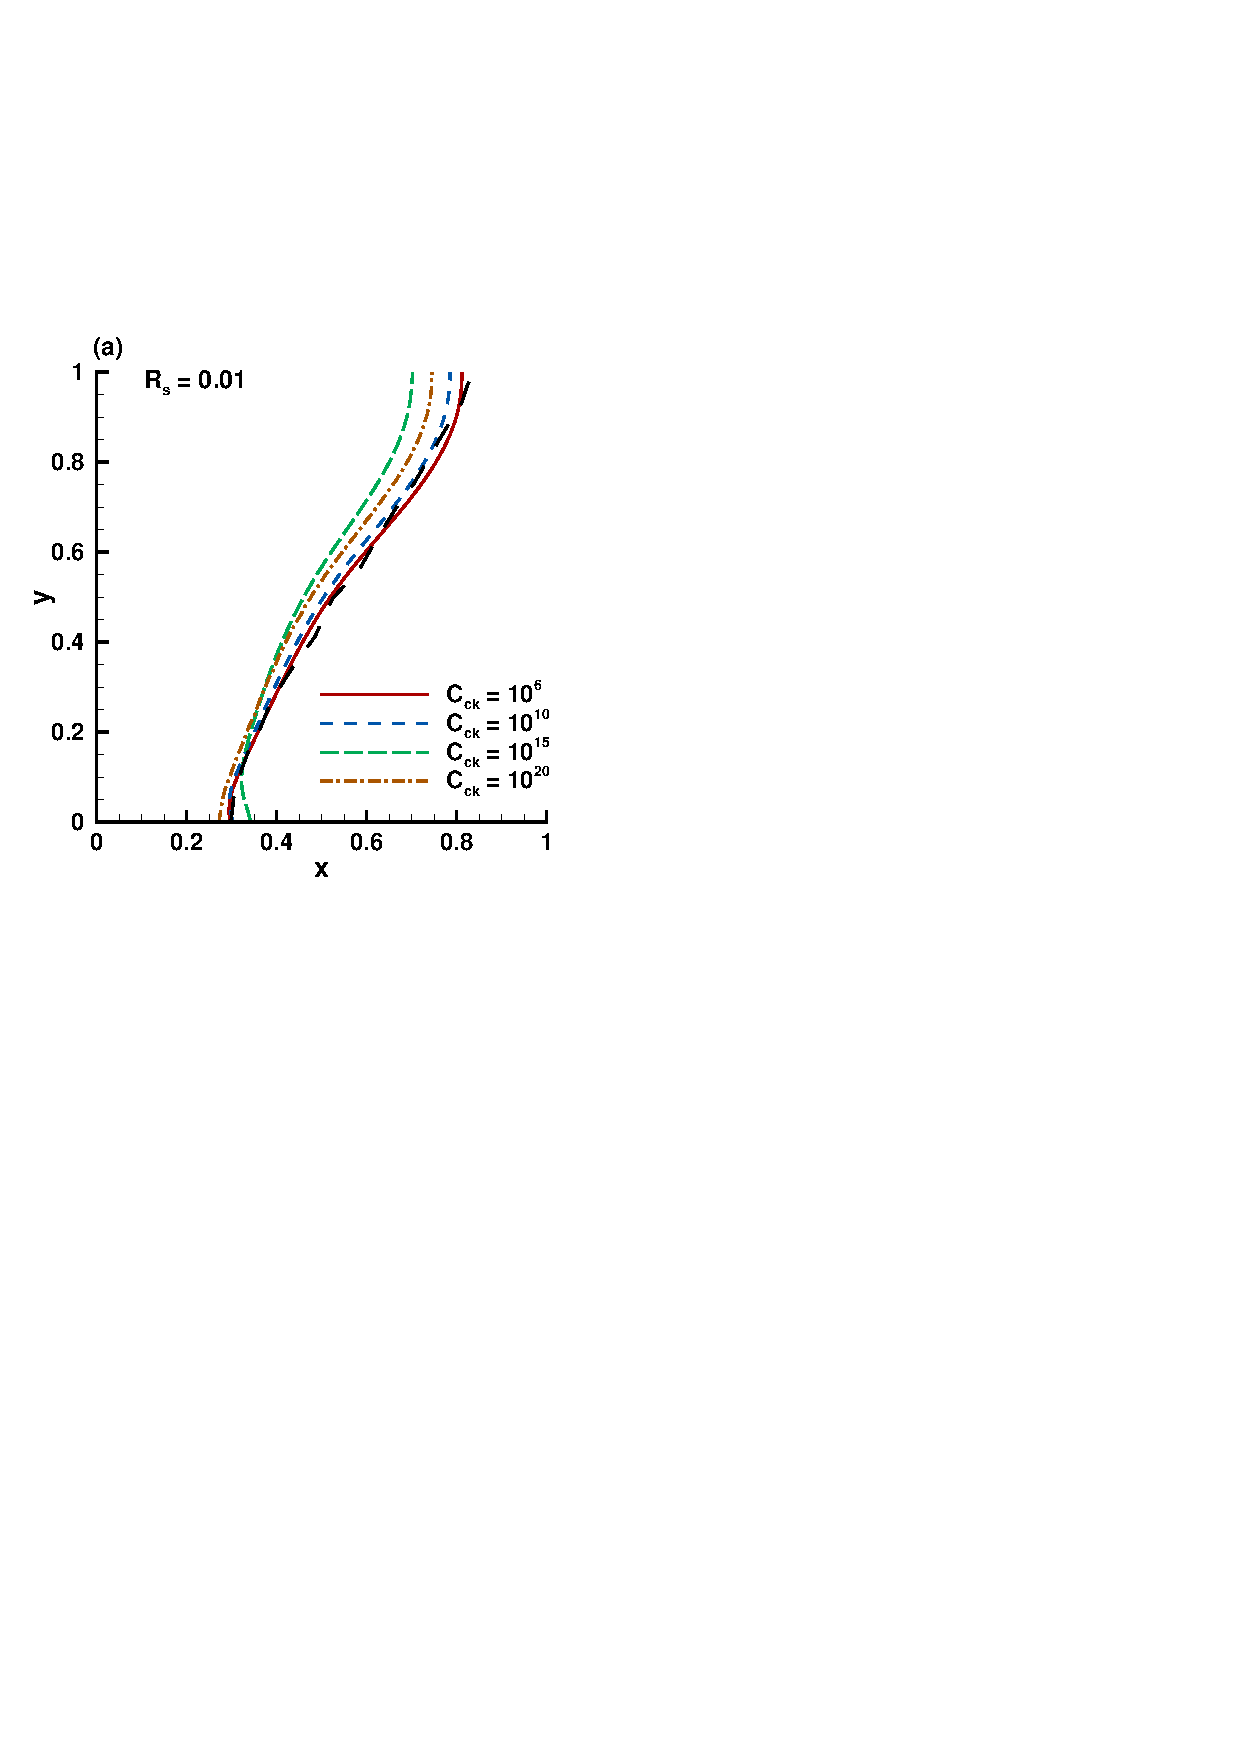
\includegraphics[width=.5\textwidth]{\figpath/Fig_cap_melting/PCM_ck_compare}
	\end{center}
	\caption{Location of the interface during the melting of the PCM using different value of $\CKC$ ranging from $10^6$ to $10^{10}$. Comparison with experimental data of \cite{Okada1984}}
	\label{fig:pcm-CK}
\end{figure}

%\newpage
%\clearpage
\subsection{Mesh adaptativity}

The use of mesh adaptation proved mandatory in the simulation of PCM melting to obtain accurate results within reasonable computational time.
For the melting case, we used five metrics intersection to adapt the mesh, based on $S^{n+1}, S^{n}, T^{n+1}, T^{n},$ and $\vec{u}^{n+1}$. To reduce the impact of the interpolation on the global accuracy for time-depending problems, we consider the metrics computed from actual (at $t_{n+1}$) and  previous (at $t_{n}$) values, for the same variable used for adaptivity (see also \cite{Belhamadia2004_S}).

The mesh adaptation strategy requires to set  the interpolation error level \texttt{errh}, the minimum edge size \texttt{hmin}, and the \texttt{adaptratio} parameter, which defines the ratio for a prescribed smoothing of the metric.
We fixe the maximum and the minimum triangle size to avoid generating too large number of nodes, and we impose also the anisotropy of the mesh to have value close to $1$.
The minimum size of triangles and the interpolation error level are set in order to capture both boundary layers region and phase-change interface.
The error level is adapted for each variable on which the metric is computed.
A default value {\em errh = 0.02} is defined for $T$ and $\vec{u}$, and {\em errh = 0.2} for $S$.

The scale for the thermal boundary layers in natural convection flow along a vertical wall is given by Eqs. \ref{eq-scale-nbd-high-Pr} and \ref{eq-corr-Low-Pr}.
For high-Prandtl simulations, the thickness of the thermal boundary layer is thinner than the viscous boundary layers. 
In our simulations, Rayleigh numbers in the range of $10^6$ to $10^8$ corresponding to Prandtl number of order of $50$, lead to a dimensionless thickness of the thermal boundary layer of order of $\delta_\theta \sim 0.01$.
Conversely, for low-Prandtl simulations the viscous boundary layer is thinner than the thermal boundary layer.
For the same range of Rayleigh numbers and Prandtl number of order of $0.1$, we have a dimensionless thickness of the viscous boundary layer of $\delta_\nu \sim 0.015$. \\
The minimum edge-length should be therefore lower than $0.01$.
Moreover, a minimum of 8 triangles should be included in the mushy zone to ensure an accurate location of the melting interface and a correct resolution of gradients.
The optimal parameters for the mesh adaptivity are given in Tab. \ref{tab-param-mesh}.
\begin{table}
   \begin{center}
      \begin{tabular}{*{5}{cl}}
               	hmin & hmax & adaptratio & errh & nbvx \\
         	\hline
         	$10^{-3}$ & $0.1$ & $1.5$ & $0.01$ & $50,000$ \\
      \end{tabular}
   \end{center}
   \caption{Parameters for the mesh adaptivity.}
   \label{tab-param-mesh}
\end{table}

%minimum edge-length is set to $h_{min} = 10^{-3}$ and the maximum edge-lenght to $h_{max} = 0.1$.
%Two values  \texttt{errh} $= 10^{-1}$ and \texttt{errh} $= 10^{-2}$, are computed and the corresponding meshes at $t=78.8$ are displayed in Fig. (FIG MAILLAGE).

\begin{figure}
	\begin{center}
		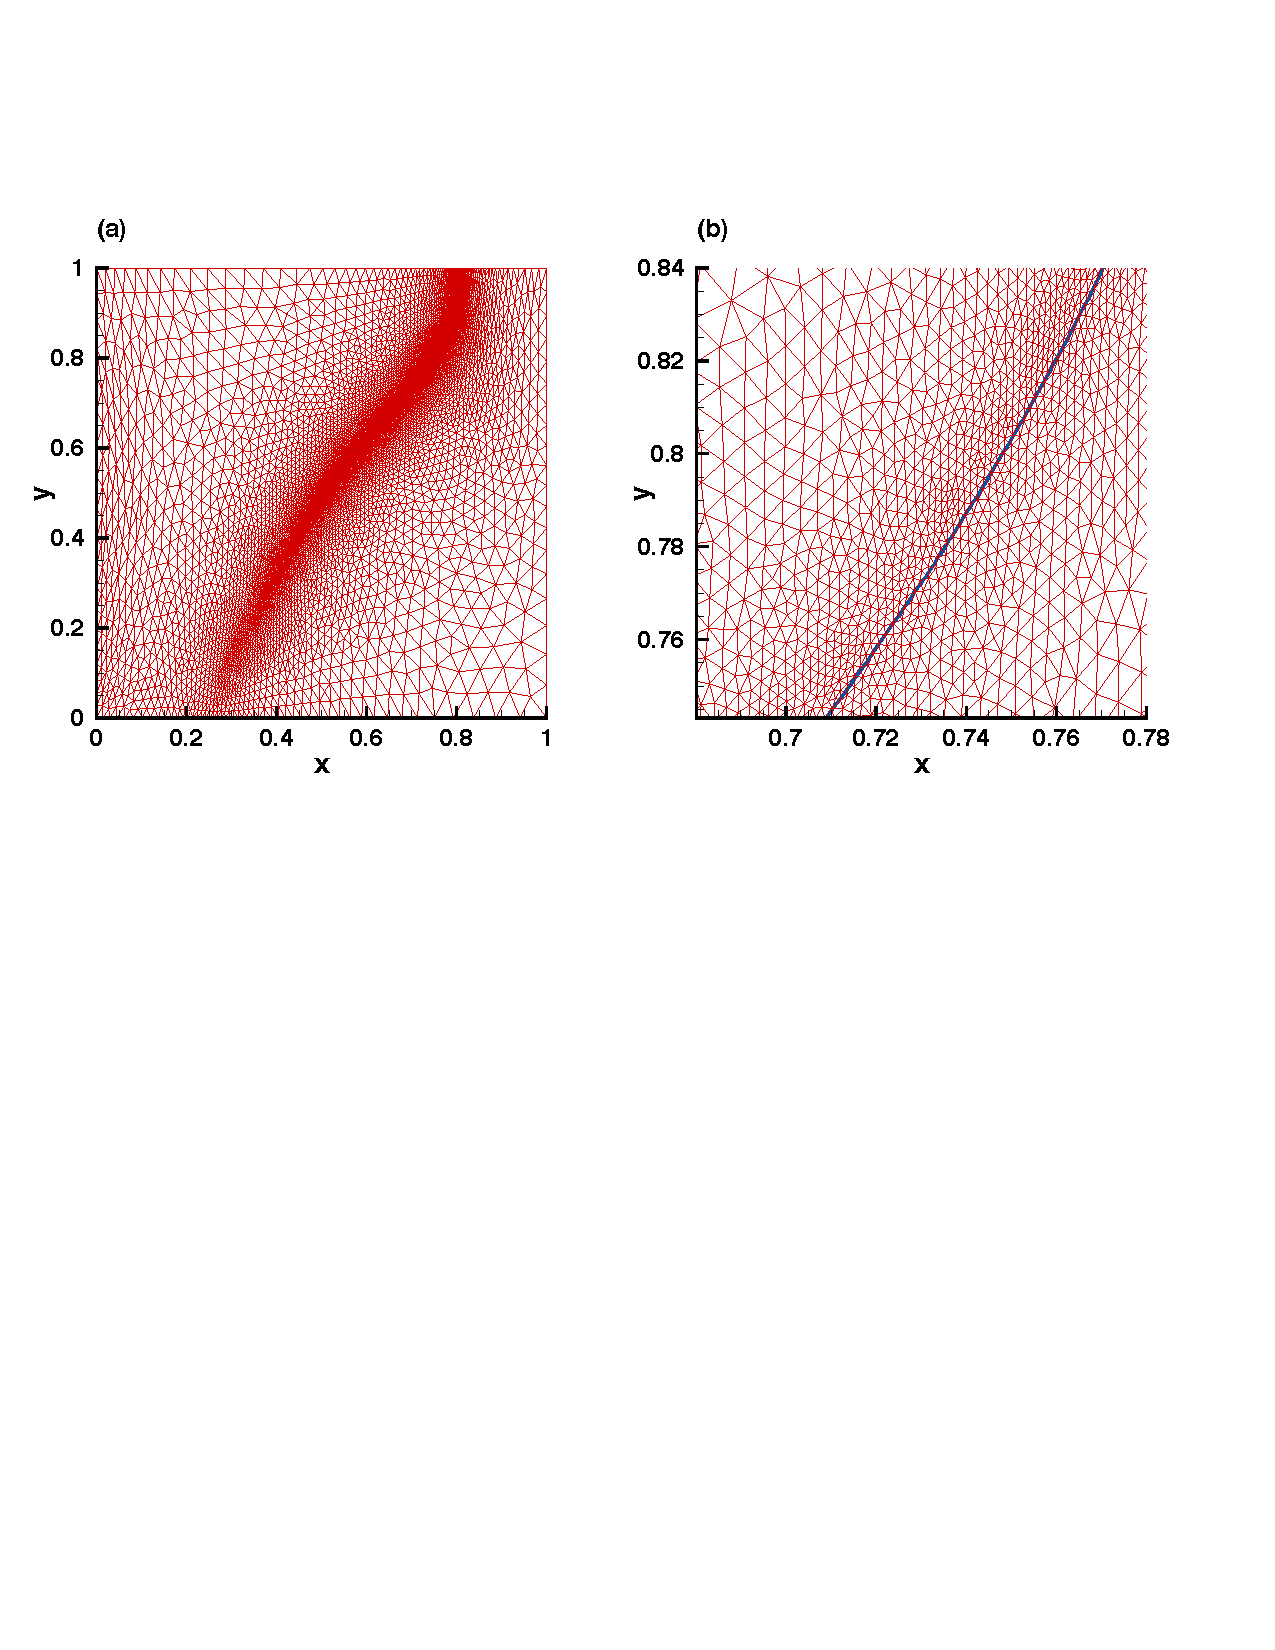
\includegraphics[width=\textwidth]{\figpath/Fig_cap_melting/Mesh_MELT}
	\end{center}
	\caption{Adapted mesh during PCM melting. (a) $4,211$ triangles: mesh is refined around the melting front $\theta=0$ and in the fluid where velocity gradients exists. (b) zoom showing the decrease of the mesh size around the temperature isoline $\theta = 0$.}
	\label{fig:pcm-mesh}
\end{figure}

Mesh adaptivity could be performed at each time step and offers a refined discretization of the regularization region where sharp gradients have to be accurately captured.  
Fig. \ref{fig:pcm-mesh} shows the adapted mesh during the melting of gallium PCM in a square cavity.
The mesh is remarkably refined around the melting front (Fig \ref{fig:pcm-mesh}b), localized by the temperature $\theta = 0$, and in the fluid region around the convection cells, while coarser mesh is applied in the solid.
The typical number of triangles of the generated adaptive mesh, during the simulation is $4,000$ triangles. 
Non-adapted grids offering the same spatial resolution everywhere inside the computational domain would have resulted in $N_t=9.94 \cdot 10^{10}$ triangles. 
Consequently, mesh adaptivity greatly helps in reducing the computational time. 

\noindent The mesh adaptivity capability to capture several interfaces is the striking feature of our method, mainly its capability to track efficiently the two solidification front during PCM solidification or the density inversion interface during the water freezing that will be discussed in Sec. \ref{sec-water-freeze}.

%\subsection{Initialization}
%The initialization is critical task in the Newton algorithm.
%For the melting process, the PCM is initially solid and the temperature should be set to a cold temperature $\theta_c$ under the temperature of fusion $\theta_f$.
%However, increasing abruptly the boundary temperature to a hot temperature $\theta_h$, over the temperature of fusion, in order to initiate the melting process is numerically complicate because of the strong temperature gradient between the wall and the PCM.
%
%A first solution is to set a very thin fluid layer of  $\delta x = 0.01$ with a constant temperature $\theta = \theta_c$.
%The drawback of this approach is that it is not physical and the evaluation of some physical properties depending on the temperature gradient at the heated wall, like the Nusselt number or the accumulated heat input, can be distorted.
%
%A second approach consist of setting an establishment regime.
%The temperature is increased smoothly over a small time steps combined with Rayleigh continuation steps.
%This approach has physical significance and is more robust when higher Rayleigh number simulations are tackled.

\newpage

\section{Melting of n-octadecane PCM in a square cavity} \label{sec: melting-2D} %: Comparison with experimental data of \cite{Okada1984}  and \cite{gong2015numerical}, and numerical data of \cite{bertrand1999melting}.}
We start the validation of our algorithm for phase-change systems by simulating the melting of n-octadecane PCM within differentially heated rectangular cavity.
Three cases are investigated: \\
\underline{\textit Benchmark $\#1$}: Experimental investigation by \cite{Okada1984} of the melting of the PCM. \\ % in enclosures of height $H=1.5$ cm. \\
%The non-dimensional parameters resulting from the physical properties of n-octadecane presented in Tab. (\ref{tab-param-PCM}) are: $\Ray = 3.27 \cdot 10^5$, $\Prd = 56.2$ and $\Ste = 0.045$ .\\
\underline{\textit Benchmark $\#2$}: Experimental and numerical study by \cite{gong2015numerical} studying PCM melting in a transparent building brick. \\ % of height $H = 15.2$ cm. \\
%The non-dimensional parameters corresponding to their experimental study are: $\Ray = 2.48 \cdot 10^8$, $\Prd = 50$ and $\Ste = 0.072$.\\
\underline{\textit Benchmark $\#3$}: Numerical comparison of various numerical methods, presented by \cite{bertrand1999melting}. \\ % considering high value of the Rayleigh number. \\
%The computed parameters are: $\Ray = 10^8$, $\Prd = 50$ and $\Ste = 0.1$.\\
%
\begin{table}[!h]
   \begin{center}
	\begin{tabular}{*{7}{c}}
  	 	&  & $\Ray$ & $\Prd$ & $\Ste$ & $\delta t$ & $V_{ref}$ \\
   		\bottomrule
   		\multirow{3}{*}{n-octadecane} & Bench $\#1$ &   $3.27 \cdot 10^5$ &  $56.2$ & $0.045$ & $10^{-1}$ & \multirow{3}{*}{$\frac{\nu_l}{H}$} \\
    		& Bench $\#2$ & $2.48 \cdot 10^8$ & $50$  & $0.072$ & $10^{-3}$ &  \\
    		& Bench $\#3$ & $10^8$ & $50$  & $0.1$ & $10^{-5}$ &  \\
    		\hline
  		 \multicolumn{2}{c}{gallium}  & $7 \cdot 10^5$ &$0.0216$  & $0.046$ & $10^{-3}$ & $\frac{\nu_l}{H}$ \\
		 \bottomrule
      \end{tabular}
   \end{center}
   \caption{Dimensionless parameters for melting of n-octadecane PCM.}
   \label{tab-param-pcm}
\end{table}

For each cases, at $t=0$ the PCM is fully solid at temperature under the temperature of fusion $\theta_h$.
Then the left wall is heated smoothly up to dimensionless temperature $\theta_h = 1$, initiating the melting. 
The right wall is held at constant dimensionless temperature $\theta_c = -0.01$.
The top and the bottom walls are adiabatic and a no-slip velocity boundary condition is used.

\begin{figure}
	\begin{center}
		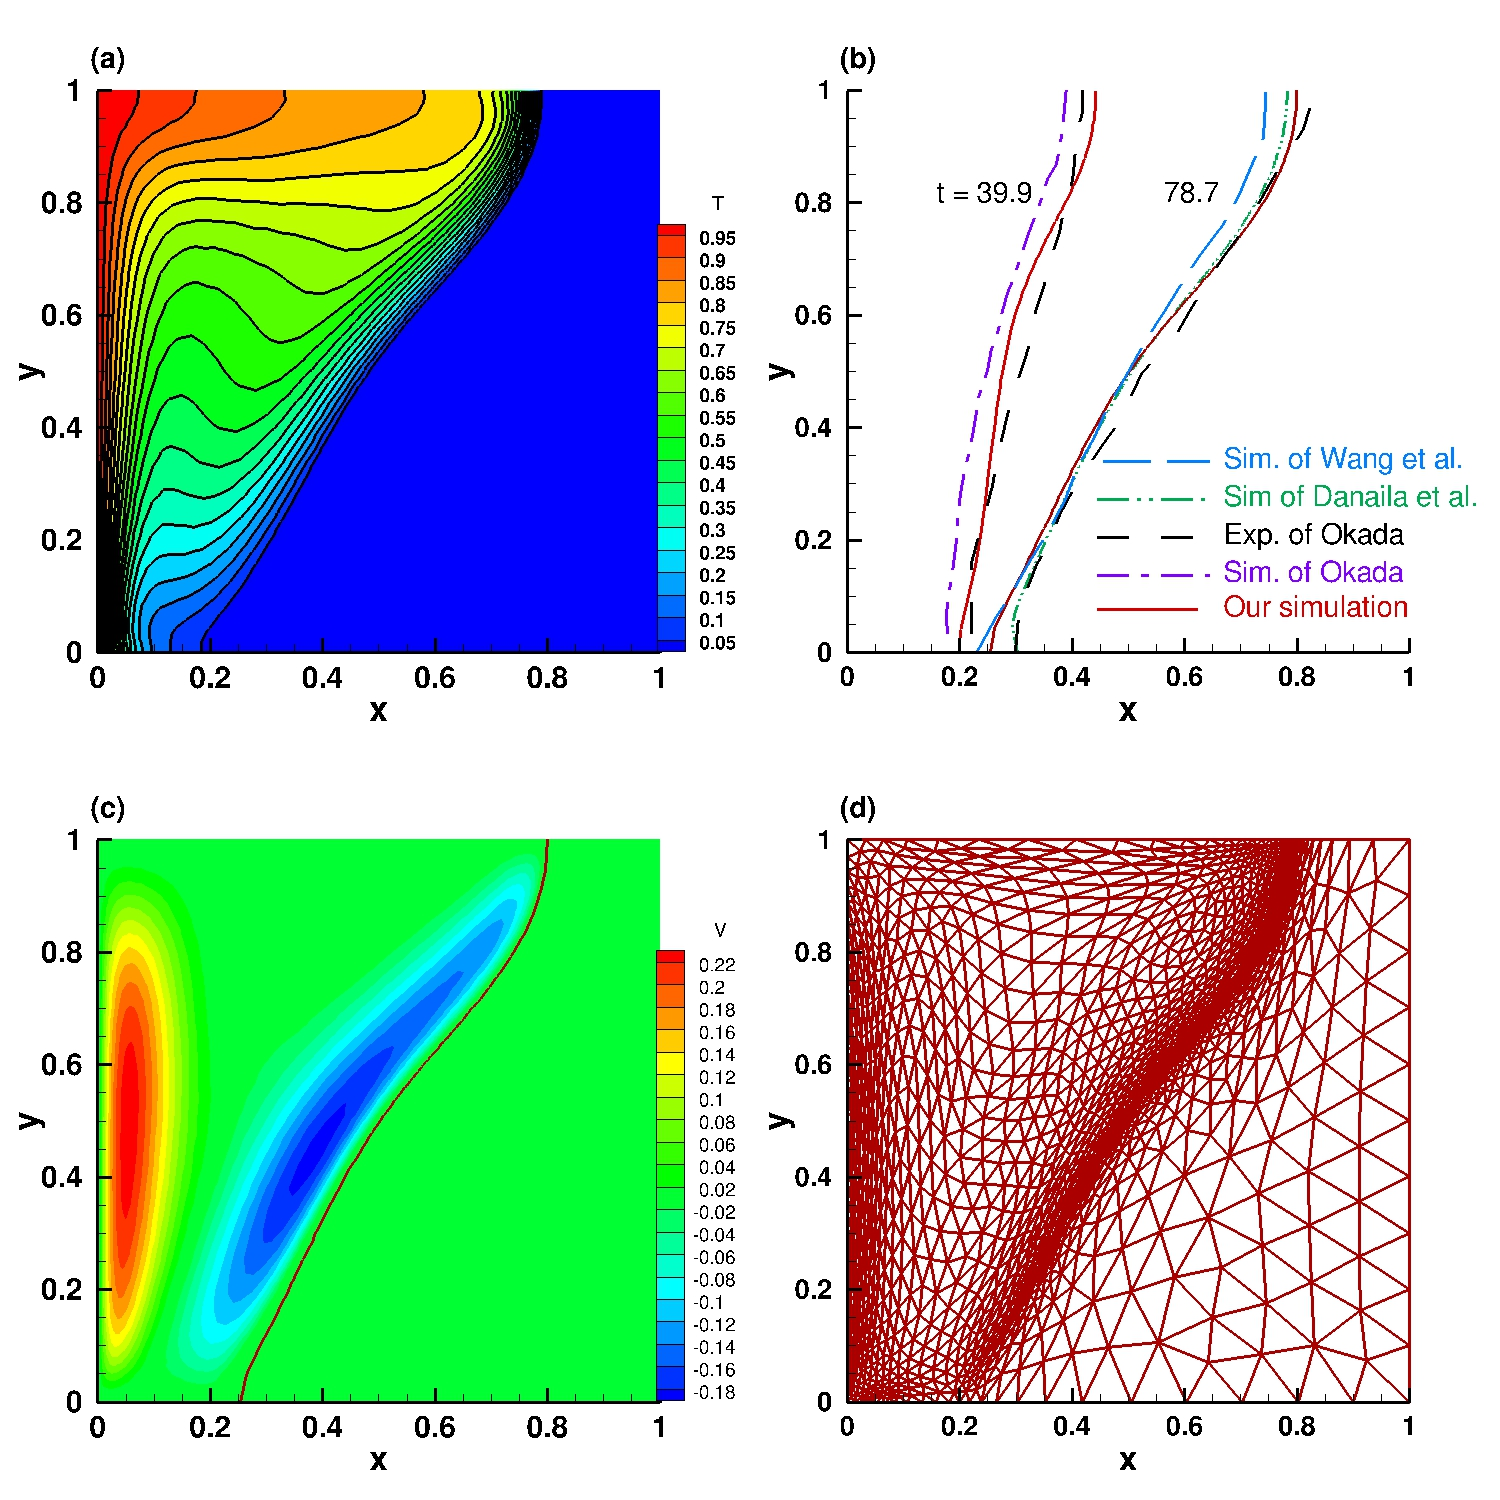
\includegraphics[width=0.9\textwidth]{\figpath/Fig_cap_melting/MELT_Okada_valid}
	\end{center}
	\caption{Benchmark $\#1$. 
	(a) Temperature isoline at $t=78.8$.
	(b) Location of the interface. Comparison with experimental data of \cite{Okada1984} and numerical solutions of \cite{dan-2014-JCP} and \cite{Wang2010} for two time instants ($t=39.9$ and $78.8$).
	(c) Vertical component of velocity field and location of the interface at $t=78.8$.
	(d) Adapted mesh with $2,900$ triangles at $t=78.8$. 
	% Benchmark 1: 
	%(b) Comparison with both experiment and simulation of \cite{gong2015numerical} for five time instants  ($\tau = 0.0002$, $0.00050$, $0.00067$, $0.00125$, $0.00252$). Benchmark 2: $\Ray = 2.48 \cdot 10^8$, $\Pr = 50$ and $\Ste = 0.072$.
	}
	\label{fig:pcm-valid}
\end{figure}

We present in Fig. \ref{fig:pcm-valid} the computed solution for Benchmark $\#1$ case.
Panel (a) shows the temperature distribution in the PCM at dimensionless time $t=78.7$ and panel (b) compare the location of the solid-liquid interface with experimental study of  \cite{Okada1984}.
%We first examine the location of the interface obtained by the current simulation.
%The comparison with the experimental results of \cite{Okada1984} is presented in Figure \ref{fig:pcm-valid}.
The experimental investigation of \cite{Okada1984} consists of a differentially heated square cavity of dimensions $1.5$ cm $\times \, 1.5$ cm. %, filled with an octadecane paraffin. 
For two particular time instants ($t=39.9$ and $t=78.7$), we could compare our results to available experimental \citep{Okada1984} and numerical \citep{Okada1984,Wang2010,dan-2014-JCP} data. \\
In the experimental set up of, the author has reported that the top of the PCM was not perfectly insulated and consequently the growth of the experimental upper melting front was delayed.
In Fig. \ref{fig:pcm-valid}(a), for the two time instants $t=39.9$ and $t=78.7$, the current work agrees well with the experimental results of \citep{Okada1984} at the bottom part of the melting front.
However, our results overestimate the location of the front in the top part of the cavity, which could be related to the experimental heat loss mentioned by the author. \\
Moreover, our results are qualitatively in a better agreement with experimental data than previously published numerical results. 
This is a direct consequence of the precise tracking of the melting front achieved by the mesh adaptivity performed at each time step.
\cite{Wang2010} have used a FV code with a fixed mesh of resolution $[60 \times 60]$, and \cite{dan-2014-JCP} have used a first order FE method with adaptive grid. \\
The vertical component of the velocity field and the resulted adapted mesh at $t=78.7$ are given in panels (c) and (d).
Thinner mesh could be observed in the boundary layer region due to the high velocity gradients, mainly near the walls, and along the interface $\theta=0$, while coarser mesh is applied in the solid region.
Panel (c) corresponds to adapted mesh with $2,900$ triangles. 


Numerical results for Benchmark $\#2$ are reported in Fig. \ref{fig:pcm-Gong}.
Panel (a) illustrates the temperature distribution in the melting PCM (the blue color denotes the solid region), the streamlines, and phase-change front.
Panel (b) compares the location of the melting front for five particular time instants: $t=0.153$, $0.347$, $0.465$, $0.869$, and $1.759$ with numerical and experimental data by \cite{gong2015numerical}.
\cite{gong2015numerical} have investigated the melting of octadecane PCM inside a transparent building brick of dimensions 
$15.2$cm$\times 3$cm.
Their numerical simulations were based on the thermal lattice Boltzmann method (TLBM), in which the natural convection got solved by the LBM and the temperature equation was solved by the finite difference scheme using enthalpy method. 
The difficulty here compared to the first validation case is the presence of a stronger natural convection flow in the fluid due to the high value of the Rayleigh number.
%The location of the melting front is compared for five particular time instants: $\tau = 0.0002$, $0.00050$, $0.00067$, $0.00125$ and $0.00252$.
%Their numerical simulation has been performed using a hybrid thermal Lattice Boltzmann method combined with an enthalpy method. 
%The location of the interface is compared for five particular time instants: $\tau = 0.0002$, $0.00050$, $0.00067$, $0.00125$ and $0.00252$.
We notice a very good agreement with the numerical and the experimental data of \cite{gong2015numerical}.

\begin{figure}
	\begin{center}
		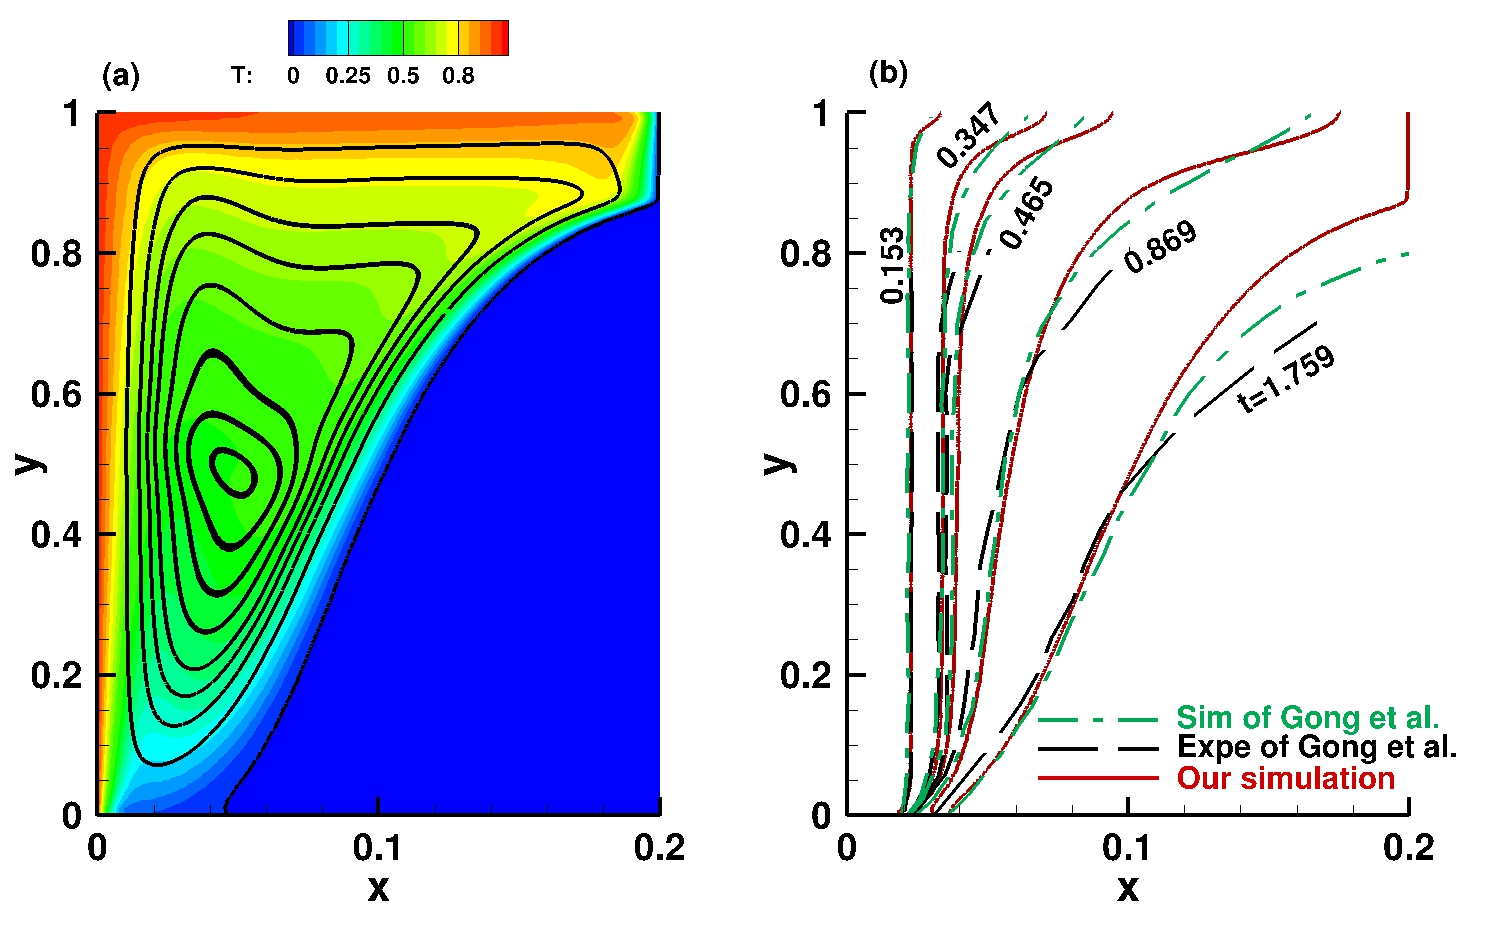
\includegraphics[width=0.95\textwidth]{\figpath/Fig_cap_melting/MELT_Gong_valid}
	\end{center}
	\caption{Benchmark $\#2$. 
	(a) Temperature distribution, streamlines, and solid-liquid interface at dimensionless time $t=1.759$.
	(b) Comparison of the location of the solid-liquid interfaces, with both experiment and simulation of \cite{gong2015numerical}, for five time instants  ($t=0.153$, $0.347$, $0.465$, $0.869$, and $1.759$).}
	\label{fig:pcm-Gong}
\end{figure}

A last validation case, for the n-octadecane PCM, is also investigated to test the robustness of the method.
\cite{bertrand1999melting} compiled results provided by five different authors (Lacroix, Le Qu{\'e}r{\'e}, Gobin-Vieira, Delannoy and Binnet-Lacroix). Results provided by these authors will be hereafter referred to as (say) 'Lacroix, from \cite{bertrand1999melting}'.
They have attempted a first comparison by taking several numerical methods to compute the basic configuration presented in this section. 
Two investigators among the five failed to predict the process and showed unrealistic behaviors (see Figs. \ref{fig Bertran} and \ref{fig-Nu-Lf-Bertran}):
Lacroix and Delannoy seem to be insufficiently converged (Fig. \ref{fig Bertran}), and Binet-Lacroix overestimates the average Nusselt number by more than $30 \%$ (Fig. \ref{fig-Nu-Lf-Bertran}).
Hence, this collection of results allows us to compare our numerical method and check whether or not realistic results are obtained for complex physical configurations.\\
We further inspect the melting front, the temporal evolution of the liquid fraction $L_f$ and the Nusselt number $N\!u$ at the left wall ($x=0$), for each of the five methods presented by \cite{bertrand1999melting}.
For the liquid fraction, the initial solid state corresponds to $L_f = 0$, while  $L_f = 1$ indicates the  complete melting of the PCM. 
%The average Nusselt number $N\!u$ at $x=0$ left boundary is defined as follows:
%\begin{equation}\label{eq-Nu}
%N\!u = \int_{0}^1 \left(\frac{\partial \theta}{\partial x}\right)_{x=0}\, dy.
%\end{equation}
%\\
\begin{figure}
	\begin{center}
		\begin{minipage}[t]{0.8\textwidth}
			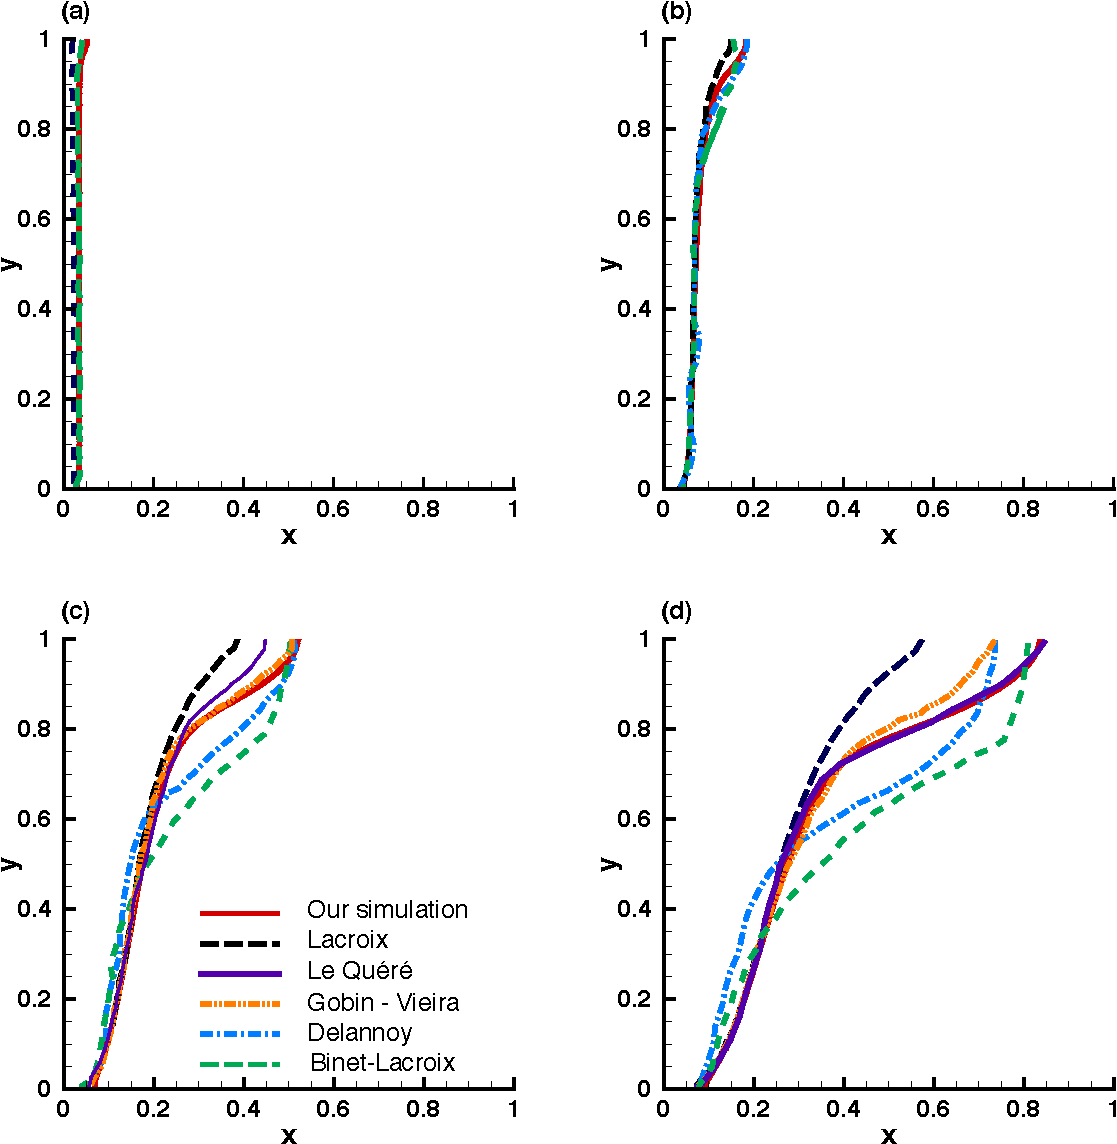
\includegraphics[width=\textwidth]{\figpath/Fig_cap_melting/fig03}
		\end{minipage}
	\end{center}
	\caption{Benchmark $\#3$. Location of the solid-liquid interface at dimensionless time (panels a to d) $t=0.25$,  $t=1$, $t=3$, and $t=5$, compared with five simulations presented by \cite{bertrand1999melting}. 
	} \label{fig Bertran}
\end{figure}
\begin{figure}
	\begin{center}
		\begin{minipage}[t]{0.8\textwidth}
			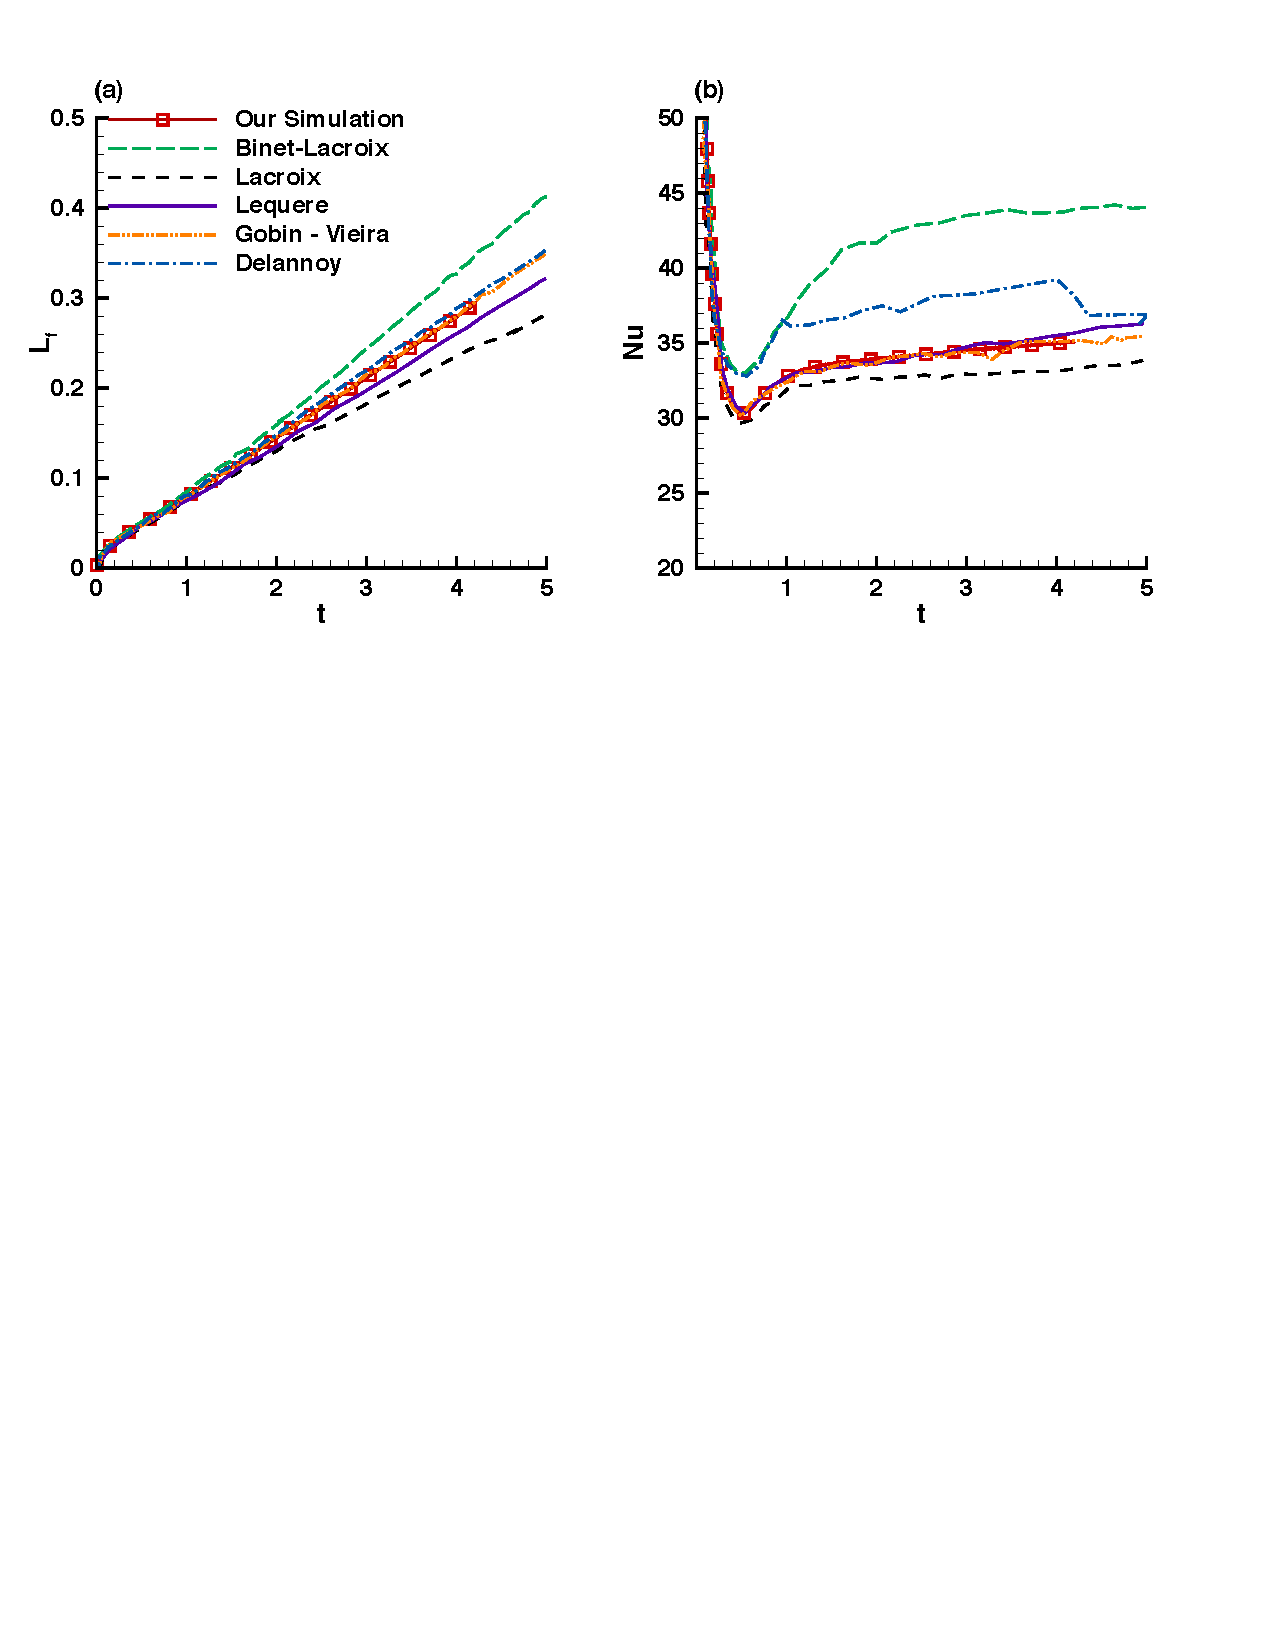
\includegraphics[width=\textwidth]{\figpath/Fig_cap_melting/Lf-Nu_Bertrand}
		\end{minipage}
	\end{center}
	\caption{Benchmark $\#3$: $\Ray = 2 \cdot 10^8$, $\Prd = 50$ and $\Ste = 0.1$. Time evolution of the liquid fraction (a) and  the  Nusselt number (b) compared with five simulations presented by \cite{bertrand1999melting}.
	} \label{fig-Nu-Lf-Bertran}
\end{figure}
The phase-change interface for four time steps, $t=0.25$,  $t=1$, $t=3$ and $t=5$ is represented in Fig. \ref{fig Bertran}.
Our results are for each case in fairly good agreement with those of Gobin and those of  Le Qu{\'e}r{\'e}.
Gobin uses a front-tracking method using a coordinate transformation with a finite volume method with a $62 \times 42$ grids.
Le Qu�r� solves a single domain model using a second order scheme with a finite volume method with a $192 \times 192$ grids  (\cite{gobin2000melting}).
The time evolution of the Nusselt number and the liquid fraction are presented in Fig. \ref{fig-Nu-Lf-Bertran}.
A very good agreement is obtained with Gobin and Le Qu{\'e}r{\'e}.
A relative difference, less than $2\%$ is noticed for the Nusselt number, and a dispersion, smaller than $4 \%$, for the melted fraction.\\
The high value of the Rayleigh number $\Ray = 10^8$ results in a very demanding numerical test.
The high velocity, inducing a very narrow thermal boundary layer can lead to unrealistic results and some numerical methods have failed.
The interest of the mesh adaptation is clearly evidenced since we  initially use only $40 \times 40$ grid points.


\section{Melting of Gallium in a rectangular cavity} \label{sec-melt-gallium}

%The observation on the melting of the gallium in a rectangular cavity was a controversy since the question if  the flow in the fluid is monocellular of multicellular was raised by \cite{dantzig1989modelling}.
The melting of the Gallium in a rectangular cavity was a controversial case since  \cite{dantzig1989modelling} raised the question 
whether  the convection in the fluid is mono-cellular or multi-cellular.
The experimental result exhibits indeed a monocellular structure, while many researchers claim this observation to be incorrect.
Prior to \cite{dantzig1989modelling} note, both experimental and numerical result support a single cell solution in the fluid phase.
Later, simulations provides solutions with multicellular flow. 
\cite{hannoun2003resolving} concluded that monocellular observation is caused by a problem of convergence of the numerical solution. It can be due to the grid size or inconsistencies in the mathematical model.

Therefore, this test case simulating the melting of the Gallium is a relevant exercice to test the consistency of our method.
To capture the very small cell during the first step of the melting, \cite{hannoun2003resolving} uses a $800 \times 1,120$ fixed grids in a rectangular domain of dimensions $6.35$ cm $\times \, 8.89$ cm. 
 \cite{hannoun2003resolving} have reported that the melting solution up to 32 s have required about $980$ CPU hours on a Compaq Alpha (667 MHz, ev67) processor.
However, a maximum of $4, 820$ triangles are necessary with our adaptive method, and only $4$ CPU hours are spent to reproduce the numerical result of \cite{hannoun2003resolving} up to the final time 280s.%, that is a ratio of $10^2$.

\begin{figure}
	\begin{center}
		\begin{minipage}[t]{\textwidth}
			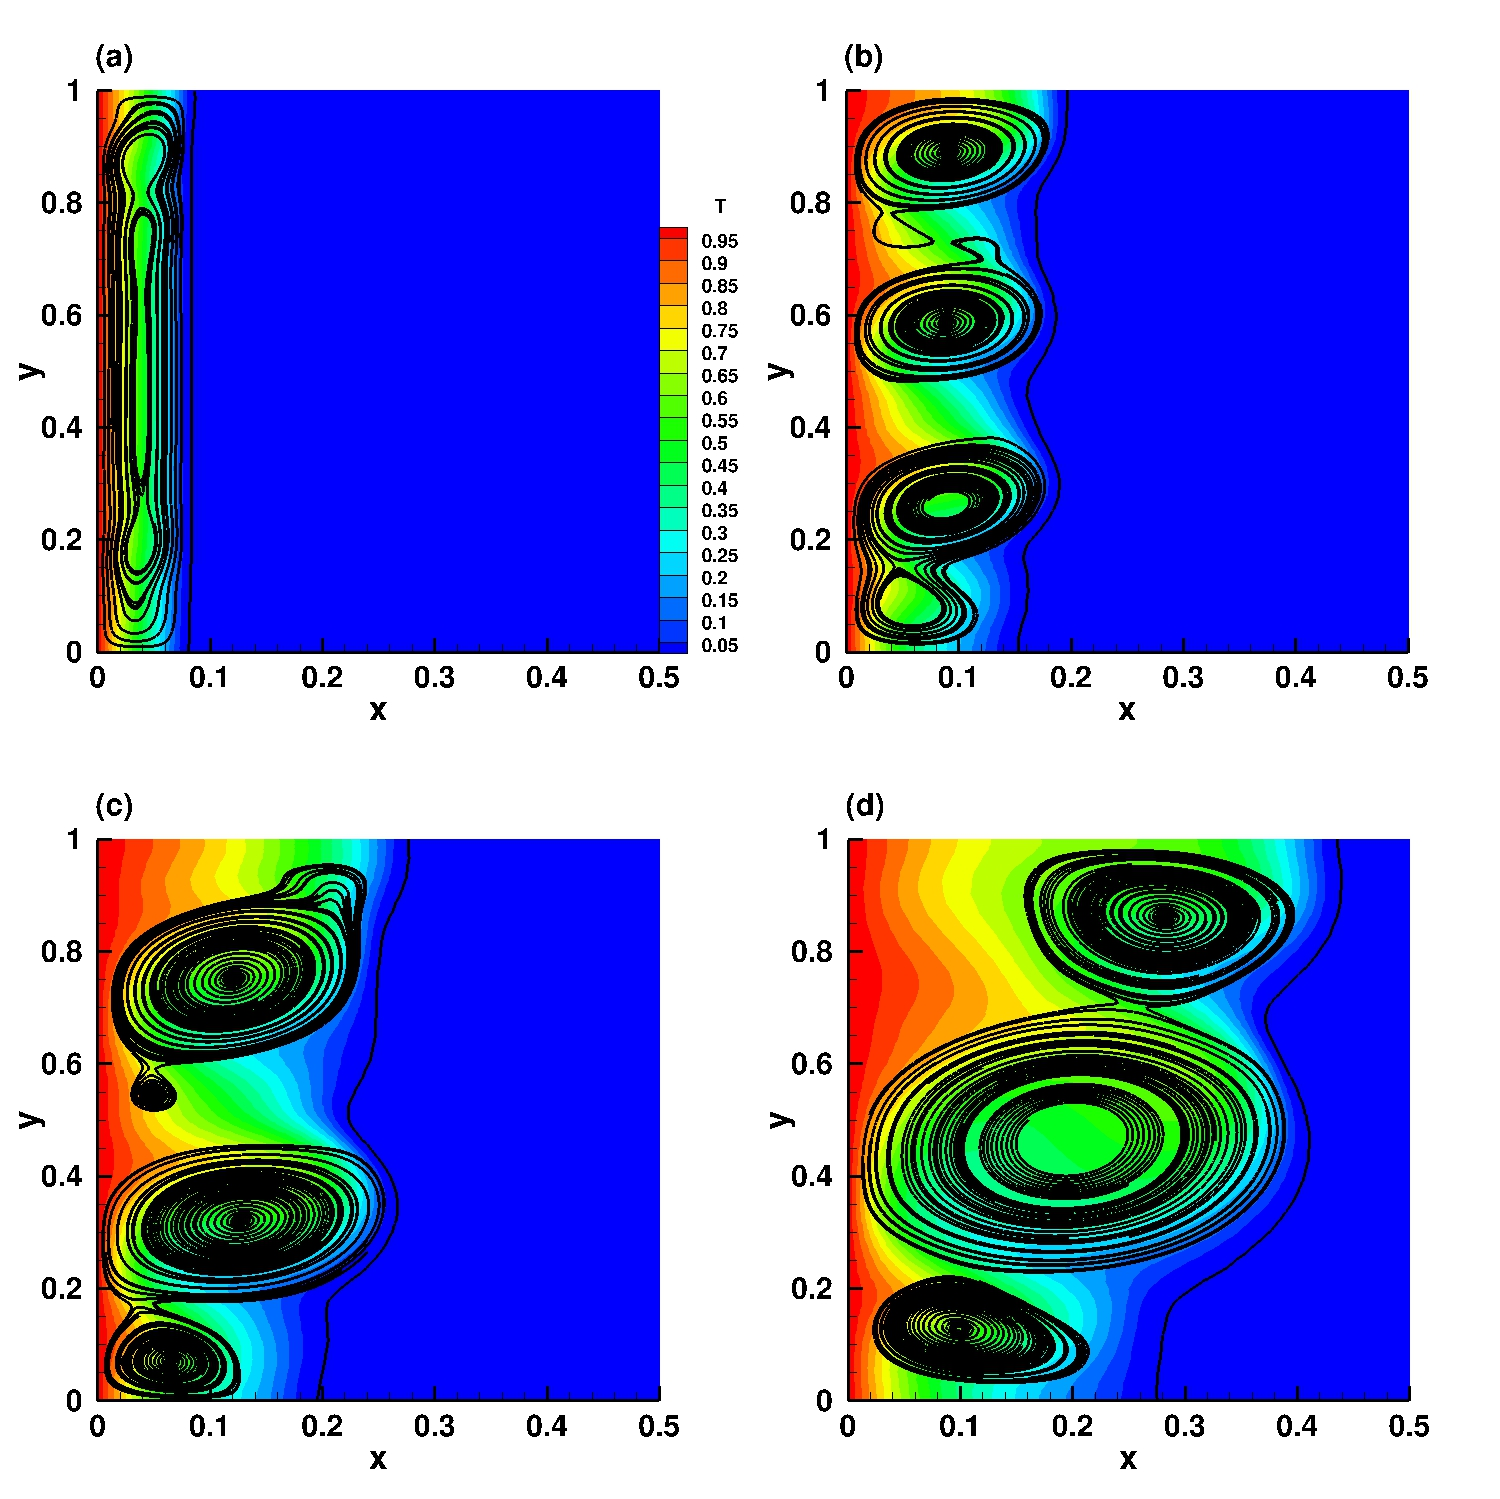
\includegraphics[width=.95\textwidth]{\figpath/Fig_cap_melting/figsCPC_11}
		\end{minipage}
	\end{center}
	\caption{PCM-Case $\#2$. Melting of Gallium: temperature field, streamlines, and melting front for dimensionless time instants (panels a to d): 
	$t = 0.0015$, $0.006$, $0.01$, and $0.019$. For a better view of the convection cells, a ratio $2:1$ was used for the axis dimensions} \label{fig-Gallium}
\end{figure}

%We consider a rectangular cavity of  $0.0635m$ height and $0.0889m$ width.
The dimensionless parameters corresponding to the gallium physical description in Tab. (\ref{tab-param-PCM}) are: $\Ray = 7 \cdot 10^5$, $\Prd = 0.0216$ and $\Ste = 0.046$.
%Gallium differs from n-octadecane since $\Prd < 1$.

The time evolution of the flow  is presented in the Fig. \ref{fig-Gallium}. Temperature filed, streamlines and position of the melting front are plotted for several time instants: $t= 0.0015$, $0.006$, $0.01$, and $0.019$.
These values were chosen to visualise the merging of convection cells in the fluid flow and correspond to physical times $20s, 85s, 155s, 280s$ in \cite{hannoun2003resolving}.
The number of rolls was considered as a validation criterion by several authors 
\citep{hannoun2003resolving,cerimele2002numerical,giangi2000melting}.
Three cells are observed  at $t=0.006$ (Fig. \ref{fig-Gallium}). The number of cells decreases later through a process of roll merging, as it was also reported  by \cite{hannoun2003resolving}. Our numerical results are in good agreement with the observations of \cite{hannoun2003resolving}, \cite{cerimele2002numerical} and \cite{giangi2000melting}.

%The time evolution of the flow is presented in the Figure \ref{fig-Gallium} with the plot of the streamlines for several physical times: $t_{\varphi} = 20s$, $32s$, $36s$, $42s$, $85s$, $155s$ and $280s$.
%These times was voluntarily chosen for they correspond to roll merging.
%\cite{hannoun2003resolving}, \cite{cerimele2002numerical} and \cite{giangi2000melting} compare the number of rolls in the fluid flow as a validation criterion.
%Five primary cells are captured at $t=32s$ and decreases later through a process of roll merging as it is noticed by \cite{hannoun2003resolving}.
%Our numerical results are in good agreement with the observations of \cite{hannoun2003resolving}, \cite{cerimele2002numerical} and \cite{giangi2000melting}.

%\section{Melting of PCM included in different geometries: cylindrical evolving inclusions, distorted mesh and rectangular}
\section{Melting of cylindrical PCM with inner heated tubes} \label{subsec-luo}
Cases presented in Secs. \ref{sec-melt-gallium} and \ref{sec: melting-2D} considered phase change problems evolving in a simple geometry, a square cavity.
%We have simulated previously phase-change problems within rectangular cavities.
%A more complex system is studied in this section, by simulating the melting of pure PCM on multitube thermal energy storage systems.
A more complex geometry, suggested by \cite{luo2015lattice}, is simulated in this section. It consists of a cylindrical PCM of  radius $R=1$ with tube inclusions of different arrangements.
%Similar configurations were studied by \cite{luo2015lattice}. Hence we could compare our numerical results to those of \cite{luo2015lattice}.
%The interest is twofold: the geometry is challenging since is it complex and \cite{luo2015lattice} uses Lattice Boltzmann method, a microscopic model, which is different from previous validation cases.
The interest in studying this case is not solely the challenge of the complex configuration, but also the possibility to compare our results with those of \cite{luo2015lattice}, obtained using a completely different model based on the Lattice Boltzmann Method. This configuration is also interesting from a practical point of view.
\cite{agyenim2010review} pointed out that more than $70\%$ of the PCM containers used for heat storage  are using shell-tube systems.

%Cylindrical PCM of dimensionless radius $R=1$ with tube inclusions are studied.
%Shell and tube PCM are indeed most intensely used in latent heat energy storage systems.
%\cite{agyenim2010review} pointed out, in a critical review of materials used for heat storage, that more than $70\%$ of the PCM container are using the shell and the tube system.

We simulate three cases taking into account one heated tube, four heated tubes, and nine heated tubes with the same contact area.
For the one heated tube case, the radius $R_i$ of the inner tube is one-quarter of the outer tube ($R_i = R/4$), for four heated tubes $R_i = R/8$ and for nine heated tubes $R_i = R/12$.
A Dirichlet boundary condition is applied to inner tubes $\theta = \theta_h$,
and a Neumann boundary condition $\frac{\partial \theta}{\partial n} = 0 $ is used at the outers.
An homogenous Dirichlet boundary condition ($\vec u = 0$) is applied everywhere for the velocity.

We have compared for the interested $\Ray$ number the simulation of the entire domain and the half of the domain and the same results were observed.
When the entire domain is investigated however, the axisymmetry of the adapted mesh is not directly handle by the mesh adaptivity algorithm and could influence the numerical solution.
To overcome this issue, the metrics for the mesh adaptivity is computed only on the half of the domain.
In the present work, only the half of the domain is simulated since the problem is symmetric because of the low $\Ray$ number investigated.
The mesh is refined initially around inner tubes, and is dynamically adapted at each time step around the melting front and the thermal boundary layer area.
The physical parameters of the simulation are:  $\Ray = 5 \cdot 10^4$, $\Prd =0.2$ and $\Ste = 0.02$.
%The same metrics presented in \ref{sec-case1} are used for the mesh adaptation process.

%The temperature distributions for each of the three cases are shown in panels (a) to (c) of Fig. (\ref{fig-Luo-Field}).
Fig. \ref{fig-Luo-Field} shows  the temperature field and the position of the solid-liquid interface (black line) for the three configurations for time instants corresponding to the same liquid fraction $L_f=80\%$. 
%The solid-liquid interface is denoted by black line.
%We can observe first the main differences in the shape of the melting front.
%The distribution of  the inner tubes in the liquid phase influences directly the fluid motion and the shape of melting front.
%The more the number of inner tubes is the more the interface is distorted.
The distribution of  the inner tubes in the liquid phase influences directly the fluid motion and the shape of melting front.
The more the number of inner tubes, the stronger the natural convection is  in the melted PCM. 
The shape of the solid-liquid interface displays complex patterns, depending on 
the space arrangement of the inner tubes. 
This is directly linked to the effect of the fluid motion in the presence of obstacles as it was also noticed in Sec. (\ref{sec: natconv-water}).
%The natural convection in the melted PCM is strengthened with the increasing number of inner heated tubes and impacts strongly the shape of the interface.
The mesh is nicely adapted following the evolution of the melting interface, even after its separation in several distinct fronts touching the outer boundary (see Figs. \ref{fig-Luo-Field}b, c). 

To estimate the efficiency of each configuration, we plot in Fig. \ref{fig-Lf-Luo} the time evolution of the liquid fraction $L_f$. 
%The time evolution of the liquid fraction is plotted in Fig. (\ref{fig-Lf-Luo}a).
By including more heated tubes the heat transfer is enhanced, inducing a faster melting time.  
The nine-tube configurations melts $5$ times faster than the reference configuration with one tube.
Note also from Fig. \ref{fig-Lf-Luo}a  a good agreement between our results and those reported by \cite{luo2015lattice} for the evolution of the liquid fraction.
%It is manifest that the heat transfer is enhanced by the number of inner heated tubes since a faster melting time is observed: a ratio of $5.4$ is noticed from the melting time with nine and one tubes.
%The current simulation is compared with the numerical data of \cite{luo2015lattice} and a good agreement is obtained.

We also assess the effect of tubes arrangements when fixe number of heated obstacles are considered. 
With $9$ heated obstacles, three arrangements are carried out: centrosymmetric, inline and staggered arrangements.
The time evolution of the liquid fraction for nine tubes is reported in Fig. \ref{fig-Lf-Luo}b.
Centrosymmetric arrangement appears to provide a better heat transfer compared to the others.
The inline and the staggered arrangements exhibits similar trends, with a slightly faster melting rate within the inline arrangement.
The difference is explained by \cite{luo2015lattice} by the contribution of conductive heat transfer induced by the arrangements.

\begin{figure}
	\begin{center}
		\begin{minipage}[t]{\textwidth}
			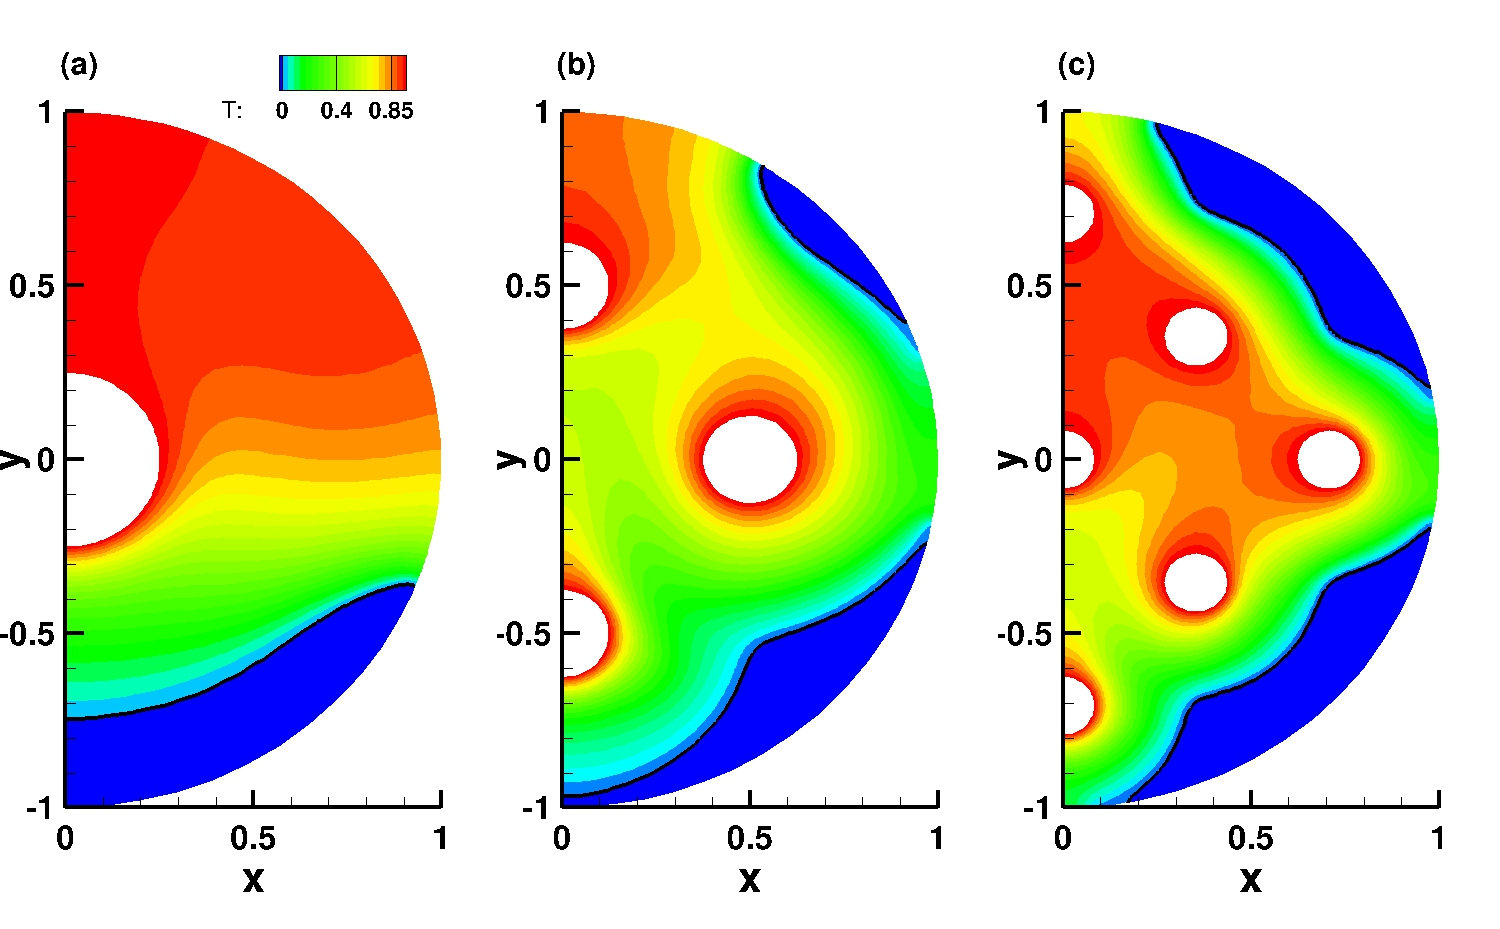
\includegraphics[width=.9\textwidth]{\figpath/Fig_cap_melting/figsCPC_09}
		\end{minipage}
	\end{center}
	\caption{PCM-Case $\#3$. Temperature fields for the melting of a cylindrical PCM with inner heated tubes. 
	Time instants corresponding to the same liquid fraction $L_f=80\%$. 
	Configurations with  (a) one tube ($t=2.5$), (b) four tunes ($t=0.99$) and (c) nine tubes ($t=0.4$).
	Melting  front are localized with black lines (only half of the domain is simulated).  
	}  \label{fig-Luo-Field}
\end{figure}

\begin{figure} 
	\begin{center} 
		\begin{minipage}[t]{\textwidth}
			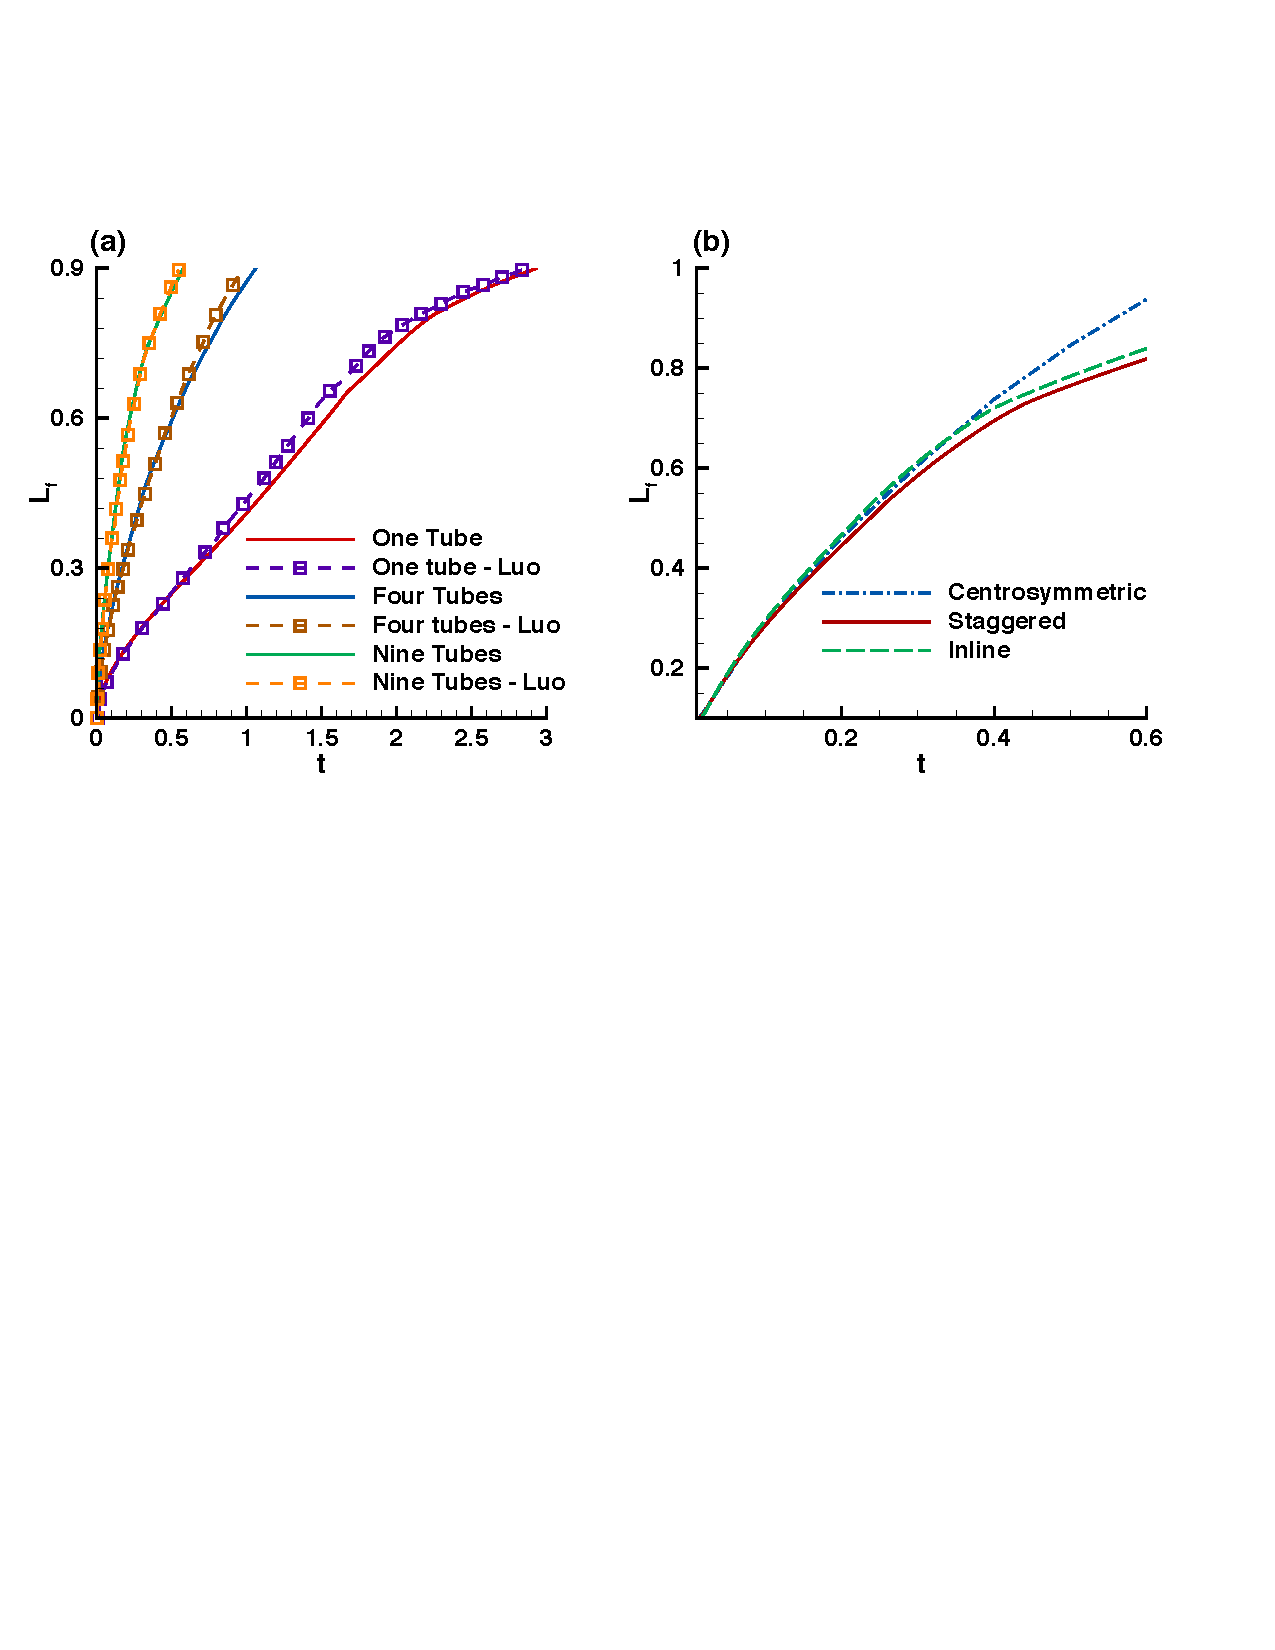
\includegraphics[width=.9\textwidth]{\figpath/Fig_cap_melting/Lf_Luo_3}
		\end{minipage}
	\end{center}
	\caption{PCM-Case $\#3$. Time evolution of the liquid fraction for one, four, and nine heated tubes. Comparison with numerical results of \cite{luo2015lattice}.} \label{fig-Lf-Luo}
\end{figure}

\section{Solid crust formation in a highly distorted mesh} \label{sec-solid-crust}
%
%\begin{figure} 
%	\begin{center}
%		\begin{minipage}[t]{\textwidth}
%			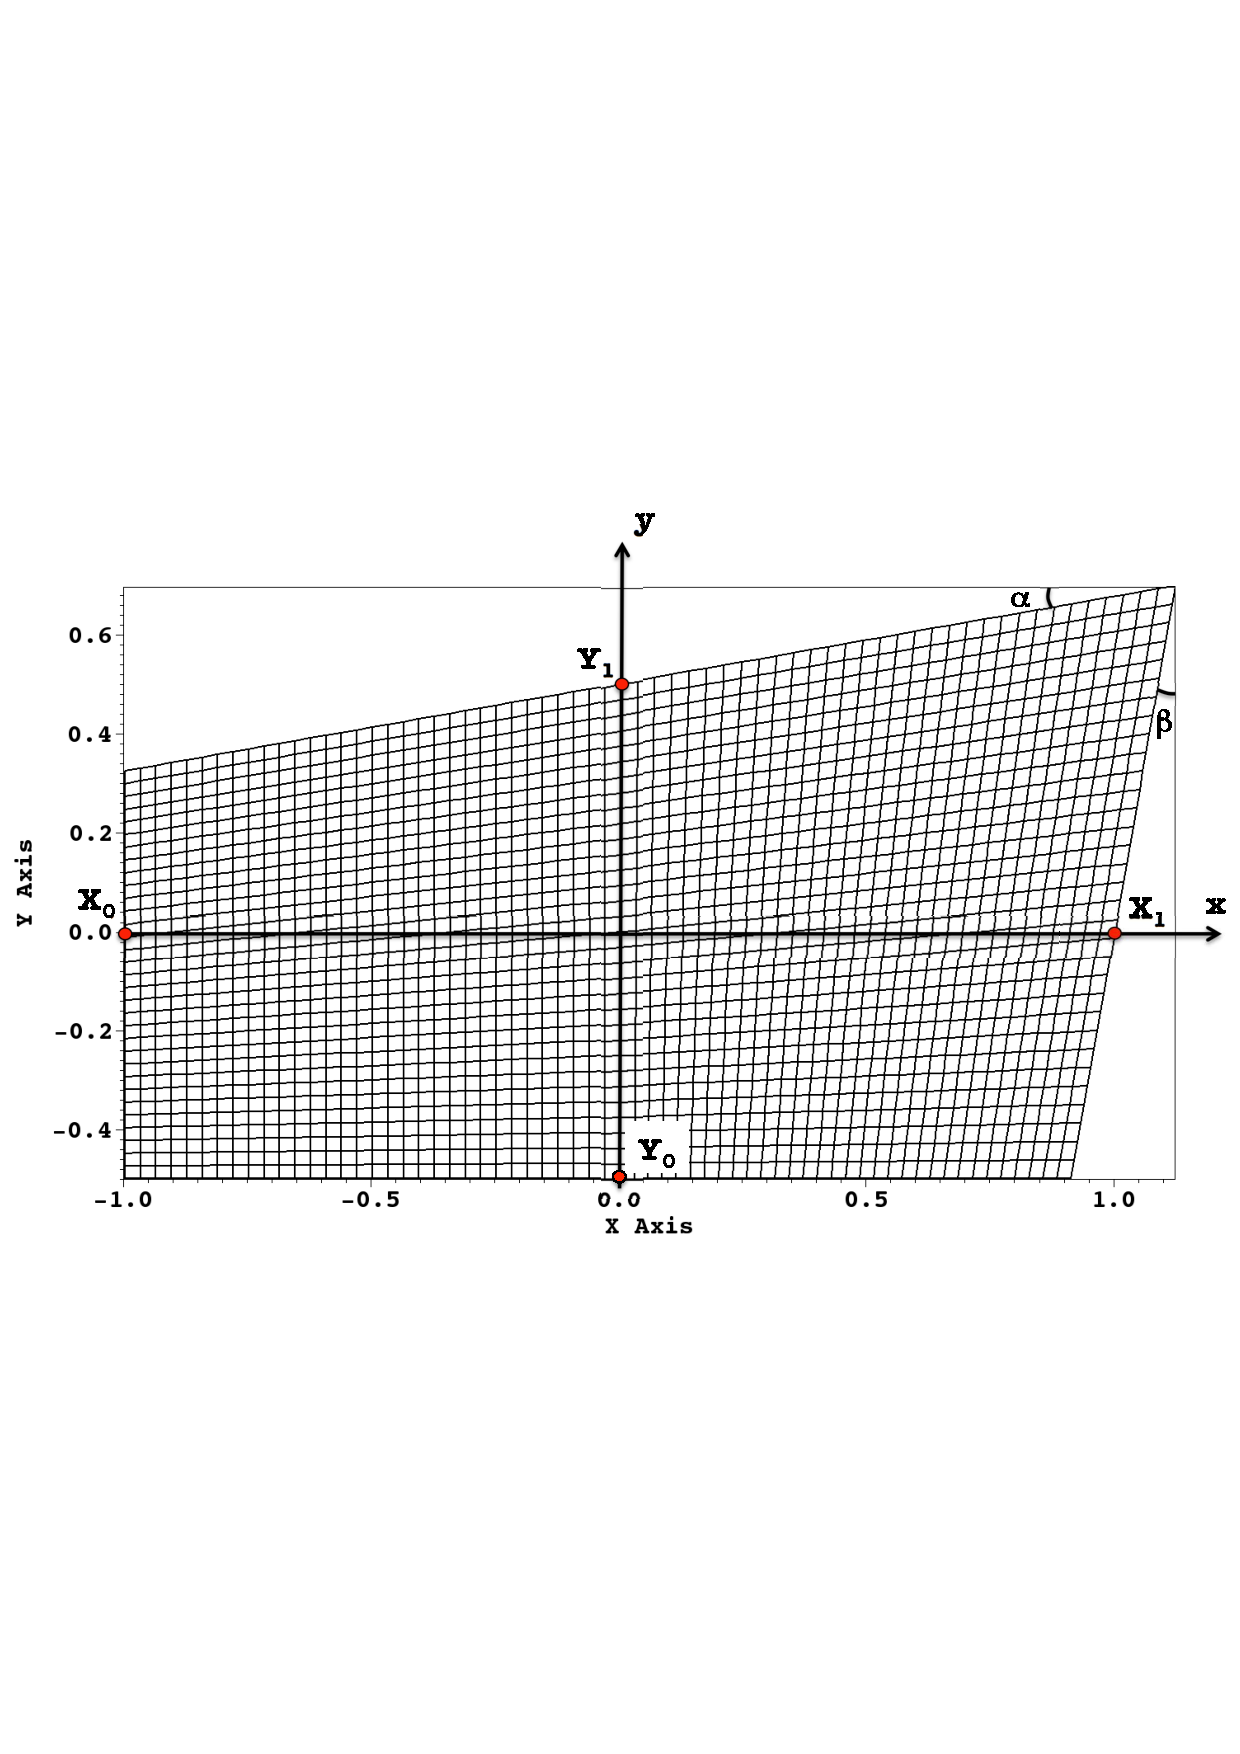
\includegraphics[width=\textwidth]{\figpath/Fig_cap_melting/DOMAIN_Nourgaliev}
%		\end{minipage}
%	\end{center}
%	\caption{Highly distorted computational domain for solid crust formation by \cite{nourgaliev2016fully}.}  \label{fig-Domain-Nourgaliev}
%\end{figure}

The solid crust formation inside a highly distorted domain, simulated by \cite{nourgaliev2016fully} is of interest in this section.
Our emphasis here is placed on the ability of our method to tackle also solidification problem, especially in irregular domain (see Fig. \ref{fig-Nourgaliev}).
%For this purpose, we use the computational domain shown in Fig. (\ref{fig-Domain-Nourgaliev}) to simulate the solidification of liquid PCM at steady its steady state.
%The six geometrical parameters, $X_0, X_1, Y_0, Y1, \alpha, \beta$ are set as follow:
%\begin{eqnarray}
%	X_0 &=& -1, \\
%	X_1 &=& 1, \\
%	Y_0 &=& -0.5, \\
%	Y_1 &=& 0.5, \\
%	\alpha &=& \beta = 20^o,
%\end{eqnarray}
%where $\alpha$ and $\beta$ define the level of stretching and distortion.

The fluid is initially motionless with an initial dimensionless temperature $\theta_i = 2$ well above the temperature of fusion.
The temperature of fusion is set to $\theta_f = 1.4$ according to \cite{nourgaliev2016fully} parameters.
It is worth noting that \cite{nourgaliev2016fully} have used $T_{ref} \ne T_f$ thus $\theta_f \ne 0$.
The left side is set at cold temperature $\theta_c = 1.39$ in the initial stage as the right wall was kept constant at a hot temperature $\theta_h = 2$, so that a steady-state natural circulation should be established. 
The cold temperature at the left wall is then dropped smoothly down to $\theta_c = 1$, below the temperature of solidification, starting the formation of a solid crust layer. 
The top and the bottom walls are adiabatics.

The dimensionless parameters of the simulation are: $\Ray = 1 \cdot 10^6$, $\Prd =0.1$ and $\Ste = 4.854$.
These investigated dimensionless parameters also allow to test the method's performance for low-Prandtl problem with high $\Ray$ and $\Ste$ numbers.
The scaling in Eq. \ref{eq-scaling-3}, which is also used by \cite{nourgaliev2016fully}, is used in the current simulation.

\begin{figure}
	\begin{center}
		\begin{minipage}[t]{\textwidth}
			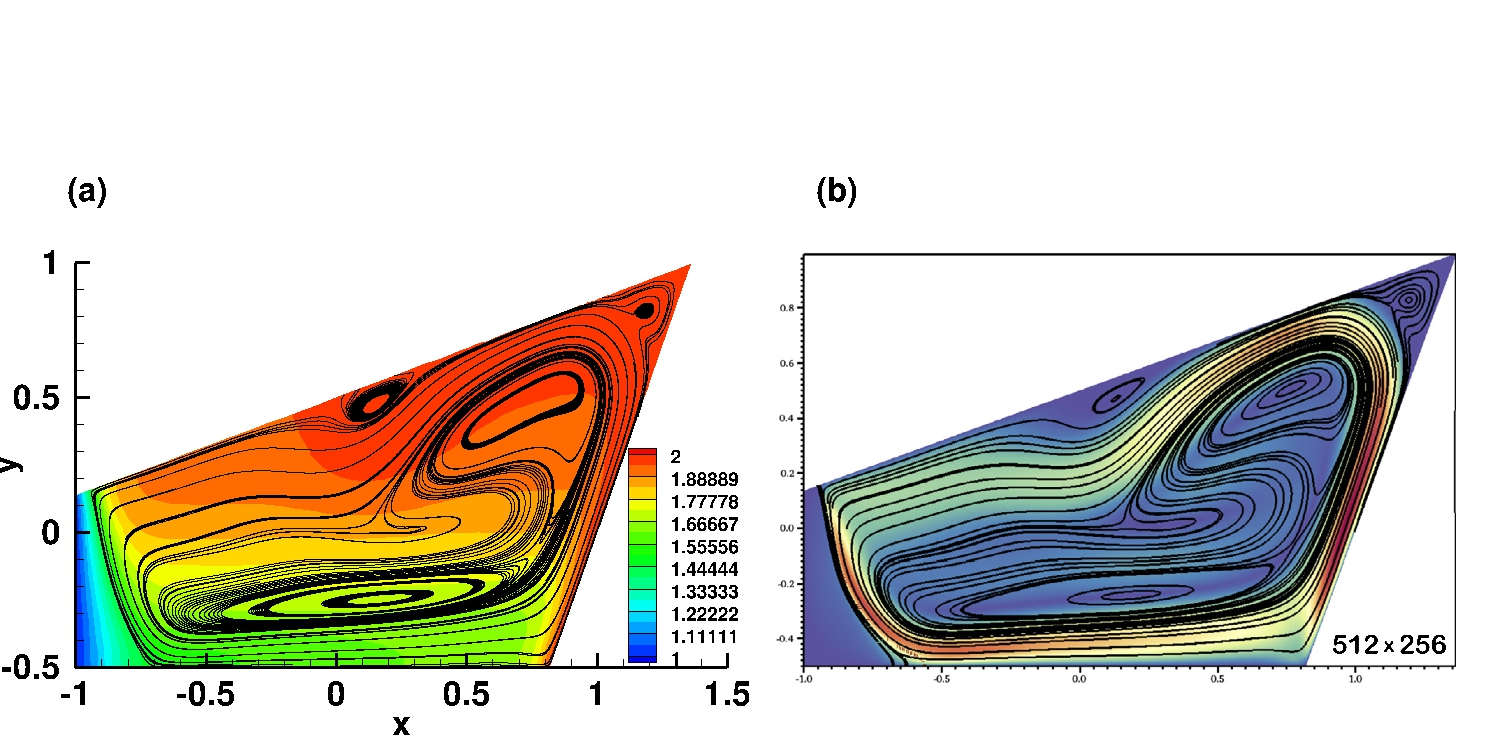
\includegraphics[width=\textwidth]{\figpath/Fig_cap_melting/figsCPC_12}
		\end{minipage}
	\end{center}
	\caption{PCM-Case $\#4$: Solid crust formation in a distorted mesh. Temperature field and streamlines of our simulation (a) and \cite{nourgaliev2016fully}  (b). } \label{fig-Nourgaliev}
\end{figure}

The temperature distribution, the streamlines as well as the melting front position are reported in Fig. \ref{fig-Nourgaliev}a and compared with the numerical results of \cite{nourgaliev2016fully},
who have used a second-order discontinuous Galerkin finite element method and a $\mu$-based technique to bring the velocity to zero in the solid region.
We are qualitatively in a fairly good agreement with \cite{nourgaliev2016fully}.
As expected, the high $\Ray$ and $\Ste$ dimensionless numbers combined with the distorted domain generate a complex vortical flow pattern in the melted PCM.
\cite{nourgaliev2016fully} have investigated a mesh convergence analysis and have concluded that a $512 \times 256$ mesh resolution is needed to get a full resolution of the five vortical structures in Fig. (\ref{fig-Nourgaliev}b),
when only $2,769$ triangles are performed in the present simulation.
This case illustrates again the power of our mesh adaptivity algorithm.

%A last assessment of the performance of our sequential code is achieved in the next section by simulating the challenging case of water freezing.


\section{Water freezing} \label{sec-water-freeze}

We consider finally the difficult case of water freezing in a square cavity. 
After achieving the convection steady pattern in the cavity (see Figure \ref{fig-T1w-isoT}), freezing starts by dropping progressively the temperature of the cold wall from $T_c=\celsm{0}$ to  $T_c=\celsm{-10}$. 
%The new boundary condition on the right cold wall is imposed by setting a very thin layer of $\delta x=0.01$ with constant temperature $\theta=\theta_c$ and zero velocity.
The dimensionless parameter describing the problem are: $\Ray=2.518084\cdot 10^{6}$, $\Prd=6.99$ and $\Ste = 0.125$.

Besides the complex fluid flow and the non-linear time evolution of the solidi-liquid interface, the code have to handle the non-linear variation of the density presented in Eq. \ref{eq-dens-nonlin}.
Moreover, one can note that in addition to the non-linear formulation of $f_B(\theta)$ in Eq. \ref{eq-fBnonlin}, the coefficient $\Ray \times 1/(\beta \delta T)$ is very large since the Boussinesq approximation imposes a value of $\beta \delta T \ll 0.01$.
Since the assumption of constant conductivity is not accurate in the frame of water phase-change, $K(\theta)$ is regularized following the smooth function:
\begin{equation}
K(T) =  1+ \frac{1}{2} \left( \frac{k_s}{k_l} - 1 \right)  \left\{
1 + \tanh \left( \frac{T_f-T}{R_{K}}\right)
\right\},
\label{eq-K-water}
\end{equation} 
with $k_s = 2.26$ and $k_l = 0.578$ the thermal conductivity of pure water in the solid and the liquid and $R_K = 0.0075$. 
%The mushy-zone definition is also slightly modified compared to the melting case.
The mushy-zone is defined as $\varepsilon_1 = 0$ and $\varepsilon_2 = 0.0075$, to ensure a very thin thickness of the mushy zone (see also \cite{dan-2014-JCP}).

Fig. \ref{fig-T2w-manip}a superimposes the experimental image from \cite{Kowalewski-1999} with our numerical results for the same physical time $t_{\varphi}=2340 [s]$. 
The flow pattern in the liquid phase also corresponds very well qualitatively to the experimental image. Since a good agreement with the experiment was sought,  the simulation was performed with very small time steps ($\delta t =10^{-4} \approx 0.15 [s]$), but still reasonable grids ($2,500$ triangles) due to the efficiency of the adaptivity algorithm.

The source term $S(\theta)$ is added to the metrics calculation presented in Sec. (\ref{sec: natconv-water}) to track the solidification front.
The mesh is thus refined along the line $\theta_m$ through the function $\Phi(\theta)$ defined in Eq. \ref{eq-Stm}, the solid-liquid interface defined by $\theta = 0$ and in the boundary layer regions.
We use also both $\Phi(\theta^n)$ and $\Phi(\theta^{n+1})$ and $S(\theta^n)$ and $S(\theta^{n+1})$ in the adaptivity procedure.
The final mesh is displayed in Fig. \ref{fig-T2w-manip}c, clearly showing that the mesh is refined along the line $\theta=\theta_m$ and the solid-liquid interface ($\theta=0$). This allows to accurately capture the structure and the extent of the two recirculating zones, features that are difficult to obtain with fixed meshes (see discrepancies described in \cite{Giangi-2000,Kowalewski-1999,Kowalewski-2003}).
As a consequence, the temperature level lines in Fig. \ref{fig-T2w-manip}d are smooth and clearly define the two interfaces in the system: the liquid-solid interface ($\theta=0$) and the density inversion interface ($\theta=0.4$) separating the two recirculating liquid regions.

\begin{figure}
	\begin{center}
		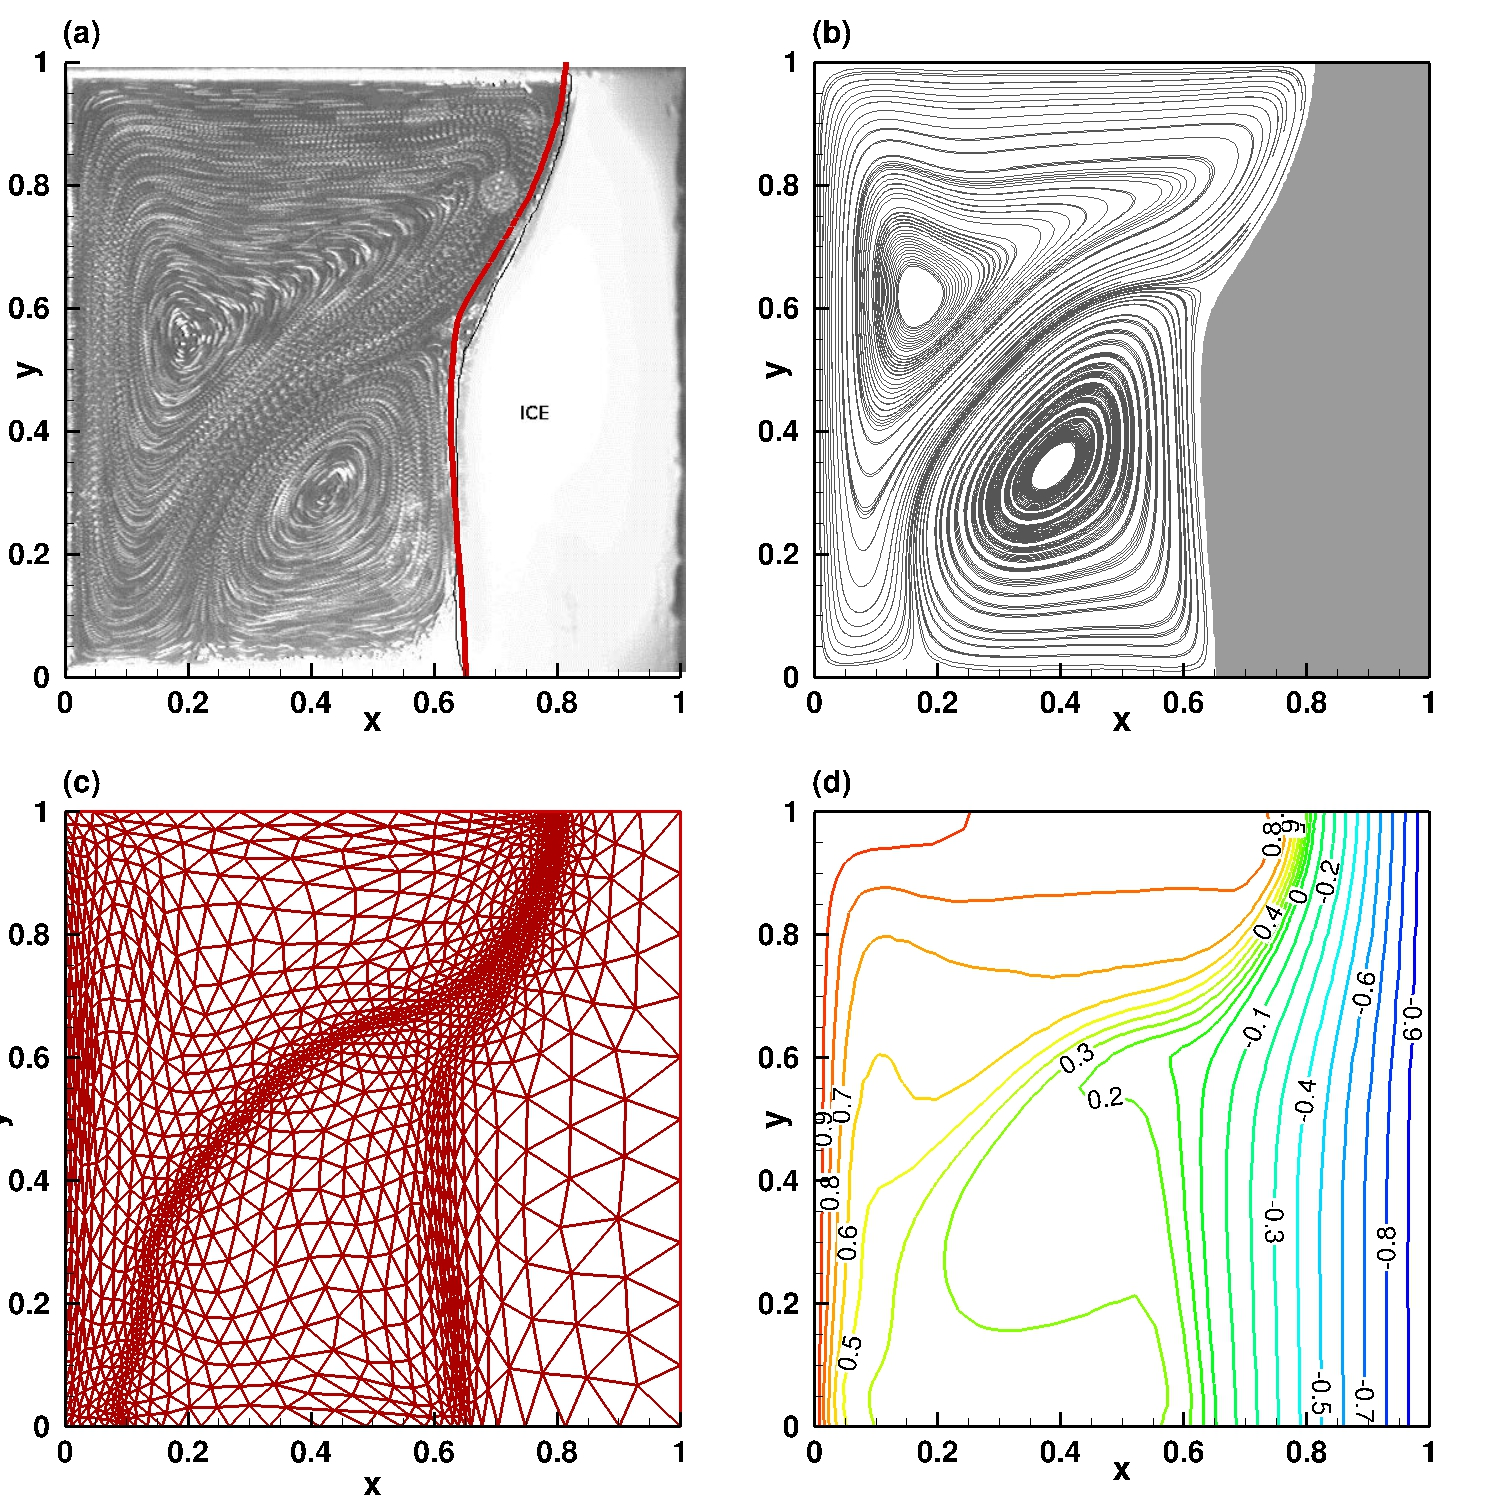
\includegraphics[width=\textwidth]{\figpath/Fig_cap_melting/figsCPC_15}
	\end{center}
	\caption{Freezing of pure water.  Configuration at (physical time) $t_{\varphi}=2340 [s]$: (a) experimental image from \cite{Kowalewski-1999}; the thick red line represents the solid-liquid interface computed with the present method (b) computed streamlines showing the two recirculating zones in the fluid phase.
	(c) finite-element mesh refined along the solid-liquid interface ($T = 0^oC$) and also along the line of maximum water density ($T = 4^oC$) (d) temperature iso-lines.}
	\label{fig-T2w-manip}
\end{figure}
%\begin{figure}
%	\begin{center}
%		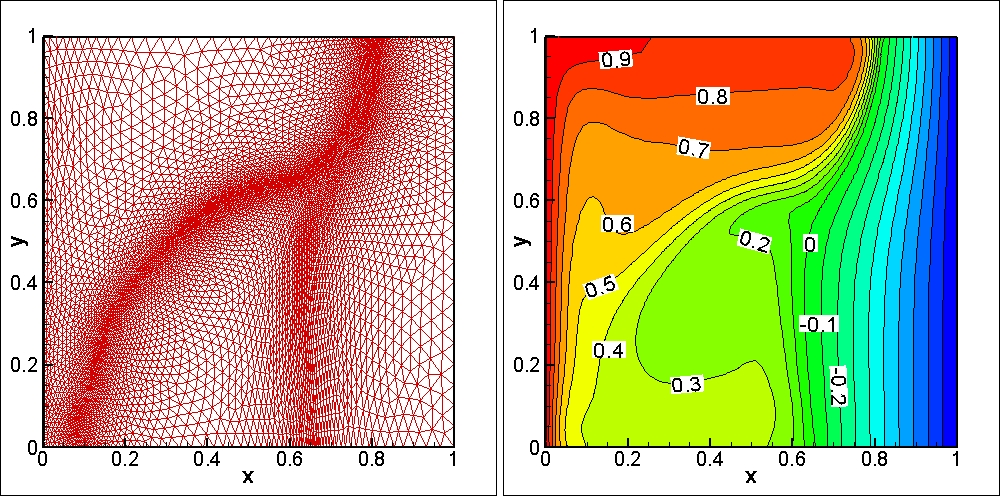
\includegraphics[width=\textwidth]{\figpath/Fig_cap_melting/danaila_fig_11.jpg}
%	\end{center}
%	\caption{Freezing of pure water.  Computed configuration at (physical time)  $t_{\varphi}=2340 [s]$: (a) finite-element mesh refined along the solid-liquid interface ($T=\celsm{0}$) and also along the line of maximum water density ($T=\celsm{4}$)  (b) temperature iso-lines.}
%	\label{fig-T2w-manipT}
%\end{figure}

\newpage
\clearpage
\section{Concluding remarks}
In this chapter, we have demonstrated our numerical method's capability to produce highly accurate solutions of difficult multiphysics problems on several geometrical configuration.
The scope of complexity involve non-linear time evolution of the solid-liquid interface that could be highly deformed by the strong convection flow in the fluid phase.
Linear and non-linear expressions of the buoyancy force was investigated.

For the linear form of $f_B$, melting of paraffin (n-octadecane) and metal (gallium) have been simulated in rectangular cavity heated from the side.
The choice of these materials is motivated by their physical properties relatively equal in both solid and liquid phases and the existence of many numerical and experimental investigation in the literature.
Comparison with existing benchmarks have shown for each cases very good agreement.
The performance of the sequential code was also proven by simulating complex geometrical configuration.
The melting of cylindrical PCM including inner heated tubes and the solidification of liquid PCM inside irregular cavity have also shown good agreement with existing numerical data.

\begin{table}[!h]
\centering
\begin{tabular}{*{4}{c}}
   \multicolumn{2}{c}{Case}  & {\small CPU time (s)} & {\small Number of triangles}  \\
  \toprule 
  \multirow{3}{*}{N-octadecane} & Bench $\#1$ & $2876.39$ & $2,900$ \\
  %\cline{2-4}
   & Bench $\#2$  & $19231$ & $4,198$ \\
   & Bench $\#3$  & $40522.7$ & $7,000$ \\
   \hline
   \multicolumn{2}{c}{Gallium} & $14621.2$ & $4,820$ \\
   \hline
  %\multicolumn{2}{c}{Cylindrical PCM} & $14621.2$ & $4,820$ \\
  \multicolumn{2}{c}{Cylindrical PCM} & $2060.42$ & $3,076$ \\
  \hline
  \multicolumn{2}{c}{Highly distorted PCM} & $6657.58$ & $2,769$ \\
%  {\small CPU time} & $2876.39$ & $40522.7$ & $2060.42$ & $14621.2$ & $6657.58$\\
%  {\small Number of triangles} & $2,900$ & $7,000$ & $3,076$ & $4,820$ & $2,769$ \\
\bottomrule
 \end{tabular}
\caption{Parameters for the cases simulating  the melting of a phase-change material.}
\label{tab-melt-cases}
\end{table}
The total CPU time and the typical number of triangles corresponding to each PCM cases are summarized in Tab. \ref{tab-melt-cases}.
Noticeable is the fact that, less than $2$ CPU hours are necessary for most of the simulations, even a sequential algorithm is used. 
The interest and the power of mesh adaptivity was highlighted by the simulation of the melting of the gallium, since only $4$ CPU hours are necessary to perform this case, while $980$ CPU hours was needed by \cite{hannoun2003resolving} using fixed-grid algorithm.

Non-linear expression of $f_B$ is considered for the solidification of pure water case. 
Besides the high $\Ray$ and $\Ste$ considered in our simulations, the efficiency of the mesh adaptivity was demonstrated by its capability to track simultaneously the interface $\theta = \theta_f$ and the line $\theta = \theta_m$ separating the two recirculating liquid regions.
Qualitative comparison with experimental image exhibits good agreement.
The vortical structures in the liquid water were accurately captured and the density inversion interface was precisely solved.
